%%%%%%%%%%%%%%%%%%%%%%%%%%%%%%%%%%%%%%%%%
% Masters/Doctoral Thesis 
% LaTeX Template
% Version 2.5 (27/8/17)
%
% This template was downloaded from:
% http://www.LaTeXTemplates.com
%
% Version 2.x major modifications by:
% Vel (vel@latextemplates.com)
%
% This template is based on a template by:
% Steve Gunn (http://users.ecs.soton.ac.uk/srg/softwaretools/document/templates/)
% Sunil Patel (http://www.sunilpatel.co.uk/thesis-template/)
%
% Template license:
% CC BY-NC-SA 3.0 (http://creativecommons.org/licenses/by-nc-sa/3.0/)
%
%%%%%%%%%%%%%%%%%%%%%%%%%%%%%%%%%%%%%%%%%

%----------------------------------------------------------------------------------------
%	PACKAGES AND OTHER DOCUMENT CONFIGURATIONS
%----------------------------------------------------------------------------------------

\documentclass[11pt,english,singlespacing,headsepline]{MastersDoctoralThesis} % The class file specifying the document structure

\usepackage[utf8]{inputenc} % Required for inputting international characters
\usepackage[T1]{fontenc} % Output font encoding for international characters

\usepackage{mathpazo} % Use the Palatino font by default

\usepackage[backend=bibtex,style=authoryear,natbib=true]{biblatex} % Use the bibtex backend with the authoryear citation style (which resembles APA)

\addbibresource{biblio.bib} % The filename of the bibliography

\usepackage[autostyle=true]{csquotes} % Required to generate language-dependent quotes in the bibliography

%----------------------------------------------------------------------------------------
%	MARGIN SETTINGS
%----------------------------------------------------------------------------------------

\geometry{
	paper=a4paper, % Change to letterpaper for US letter
	inner=2.5cm, % Inner margin
	outer=3.8cm, % Outer margin
	bindingoffset=.5cm, % Binding offset
	top=1.5cm, % Top margin
	bottom=1.5cm, % Bottom margin
	%showframe, % Uncomment to show how the type block is set on the page
}

%----------------------------------------------------------------------------------------
%	THESIS INFORMATION
%----------------------------------------------------------------------------------------

\thesistitle{Evaluation of Optical Aberrations using Phase Diversity} % Your thesis title, this is used in the title and abstract, print it elsewhere with \ttitle
\supervisor{Dr. Laurent \textsc{Jolissaint}} % Your supervisor's name, this is used in the title page, print it elsewhere with \supname
\cosupervisor{Dr. Jean-Paul \textsc{Kneib}}
\examiner{} % Your examiner's name, this is not currently used anywhere in the template, print it elsewhere with \examname
\degree{Master in Applied Physics} % Your degree name, this is used in the title page and abstract, print it elsewhere with \degreename
\author{Jordan \textsc{Voirin}} % Your name, this is used in the title page and abstract, print it elsewhere with \authorname
\addresses{} % Your address, this is not currently used anywhere in the template, print it elsewhere with \addressname

\subject{Optical Physics} % Your subject area, this is not currently used anywhere in the template, print it elsewhere with \subjectname
\keywords{} % Keywords for your thesis, this is not currently used anywhere in the template, print it elsewhere with \keywordnames
\university{\href{http://www.epfl.ch}{Ecole Polytechnique Fédérale de Lausanne}} % Your university's name and URL, this is used in the title page and abstract, print it elsewhere with \univname
\department{\href{http://sb.epfl.ch}{Basic Sciences}} % Your department's name and URL, this is used in the title page and abstract, print it elsewhere with \deptname
\group{\href{http://lastro.epfl.ch/}{Astrophysics laboratory}} % Your research group's name and URL, this is used in the title page, print it elsewhere with \groupname
\faculty{\href{http://sb.epfl.ch/physics}{Physics}} % Your faculty's name and URL, this is used in the title page and abstract, print it elsewhere with \facname

\AtBeginDocument{
\hypersetup{pdftitle=\ttitle} % Set the PDF's title to your title
\hypersetup{pdfauthor=\authorname} % Set the PDF's author to your name
\hypersetup{pdfkeywords=\keywordnames} % Set the PDF's keywords to your keywords
}

%parameter to type code

\definecolor{forestgreen}{rgb}{0.0, 0.27, 0.13}
\lstset{frame=tb,
  language=Python,
  aboveskip=3mm,
  belowskip=3mm,
  showstringspaces=false,
  columns=flexible,
  basicstyle={\small\ttfamily},
  numbers=left, numbersep=5pt,
  numberstyle=\tiny\color{gray},
  keywordstyle=\color{blue},
  commentstyle=\color{forestgreen},
  stringstyle=\color{magenta},
  breaklines=true,
  breakatwhitespace=true,
  tabsize=3
}

%for description list to be aligned with the text
\setlist[description]{leftmargin=0cm}

\begin{document}

\frontmatter % Use roman page numbering style (i, ii, iii, iv...) for the pre-content pages

\pagestyle{plain} % Default to the plain heading style until the thesis style is called for the body content

%----------------------------------------------------------------------------------------
%	TITLE PAGE
%----------------------------------------------------------------------------------------

\begin{titlepage}
\begin{center}

%\vspace*{.05\textheight}

\includegraphics[scale=.25]{Logo/Logo_EPFL.png} \hfill

\includegraphics[scale=.625]{Logo/HEIG-VD_Logo.png} \\[1cm]

{\scshape\LARGE \univname\par}\vspace{1.2cm} % University name
\textsc{\Large Master Thesis}\\[0.5cm] % Thesis type

\HRule \\[0.4cm] % Horizontal line
{\huge \bfseries \ttitle\par}\vspace{0.4cm} % Thesis title
\HRule \\[1.5cm] % Horizontal line
 
\begin{minipage}[t]{0.4\textwidth}
\begin{flushleft} \large
\emph{Author:}\\
{\authorname} % Author name - remove the \href bracket to remove the link
\end{flushleft}
\end{minipage}
\begin{minipage}[t]{0.4\textwidth}
\begin{flushright} \large
\emph{Supervisors:} \\
\href{https://www.researchgate.net/profile/Laurent_Jolissaint/publications}{\supname}\\ % Supervisor name - remove the \href bracket to remove the link  
\href{https://people.epfl.ch/cgi-bin/people?id=222189&op=bio}{\cosupname}
\end{flushright}
\end{minipage}\\[3cm]
 
\vfill

\large \textit{A thesis submitted in fulfillment of the requirements\\ for the degree of \degreename}\\[0.3cm] % University requirement text
\textit{in the}\\[0.4cm]
\groupname\\\deptname\\[2cm] % Research group name and department name
 
\vfill

{\large \today}\\[3cm] % Date
%\includegraphics{Logo} % University/department logo - uncomment to place it
 
\vfill
\end{center}
\end{titlepage}

%----------------------------------------------------------------------------------------
%	DECLARATION PAGE
%----------------------------------------------------------------------------------------

\begin{declaration}
\addchaptertocentry{\authorshipname} % Add the declaration to the table of contents
\noindent I, \authorname, declare that this thesis titled, \enquote{\ttitle} and the work presented in it are my own. I confirm that:

\begin{itemize} 
\item This work was done wholly or mainly while in candidature for a research degree at this University.
\item Where any part of this thesis has previously been submitted for a degree or any other qualification at this University or any other institution, this has been clearly stated.
\item Where I have consulted the published work of others, this is always clearly attributed.
\item Where I have quoted from the work of others, the source is always given. With the exception of such quotations, this thesis is entirely my own work.
\item I have acknowledged all main sources of help.
\item Where the thesis is based on work done by myself jointly with others, I have made clear exactly what was done by others and what I have contributed myself.\\
\end{itemize}
 
\noindent Signed:\\
\rule[0.5em]{25em}{0.5pt} % This prints a line for the signature
 
\noindent Date:\\
\rule[0.5em]{25em}{0.5pt} % This prints a line to write the date
\end{declaration}

\cleardoublepage

%----------------------------------------------------------------------------------------
%	QUOTATION PAGE
%----------------------------------------------------------------------------------------

\vspace*{0.2\textheight}

\noindent\enquote{\itshape For the sake of persons of ... different types, scientific truth should be presented in different forms, and should be regarded as equally scientific, whether it appears in the robust form and the vivid coloring of a physical illustration, or in the tenuity and paleness of a symbolic expression. }\bigbreak

\hfill James Clerk Maxwell

%----------------------------------------------------------------------------------------
%	ABSTRACT PAGE
%----------------------------------------------------------------------------------------

%\begin{abstract}
%\addchaptertocentry{\abstractname} % Add the abstract to the table of contents
%The Thesis Abstract is written here (and usually kept to just this page). The page is kept centered vertically so can expand into the blank space above the title too\ldots
%\end{abstract}

%----------------------------------------------------------------------------------------
%	ACKNOWLEDGEMENTS
%----------------------------------------------------------------------------------------

\begin{acknowledgements}
\addchaptertocentry{\acknowledgementname} % Add the acknowledgements to the table of contents
The acknowledgments and the people to thank go here, don't forget to include your project advisor\ldots
\end{acknowledgements}

%----------------------------------------------------------------------------------------
%	LIST OF CONTENTS/FIGURES/TABLES PAGES
%----------------------------------------------------------------------------------------

\tableofcontents % Prints the main table of contents

\listoffigures % Prints the list of figures

\listoftables % Prints the list of tables

%----------------------------------------------------------------------------------------
%	ABBREVIATIONS
%----------------------------------------------------------------------------------------

%\begin{abbreviations}{ll} % Include a list of abbreviations (a table of two columns)
%\textbf{FWHM} & \textbf{F}ull \textbf{W}idth \textbf{H}alf \textbf{M}aximum\\
%\textbf{PD} & \textbf{P}hase \textbf{D}iversity\\
%\textbf{PSF} & \textbf{P}oint \textbf{S}read \textbf{F}unction\\
%\textbf{WFS} & \textbf{W}ave\textbf{F}ront \textbf{S}ensor\\
%
%\end{abbreviations}

%----------------------------------------------------------------------------------------
%	PHYSICAL CONSTANTS/OTHER DEFINITIONS
%----------------------------------------------------------------------------------------

%\begin{constants}{lr@{${}={}$}l} % The list of physical constants is a three column table
%
%% The \SI{}{} command is provided by the siunitx package, see its documentation for instructions on how to use it
%
%Speed of Light & $c_{0}$ & \SI{2.99792458e8}{\meter\per\second} (exact)\\
%%Constant Name & $Symbol$ & $Constant Value$ with units\\
%
%\end{constants}

%----------------------------------------------------------------------------------------
%	SYMBOLS
%----------------------------------------------------------------------------------------

%\begin{symbols}{lll} % Include a list of Symbols (a three column table)
%
%$a$ & distance & \si{\meter} \\
%$P$ & power & \si{\watt} (\si{\joule\per\second}) \\
%%Symbol & Name & Unit \\
%
%\addlinespace % Gap to separate the Roman symbols from the Greek
%
%$\omega$ & angular frequency & \si{\radian} \\
%
%\end{symbols}

%----------------------------------------------------------------------------------------
%	DEDICATION
%----------------------------------------------------------------------------------------

%\dedicatory{For/Dedicated to/To my\ldots} 

%----------------------------------------------------------------------------------------
%	THESIS CONTENT - CHAPTERS
%----------------------------------------------------------------------------------------

\mainmatter % Begin numeric (1,2,3...) page numbering

\pagestyle{thesis} % Return the page headers back to the "thesis" style

% Include the chapters of the thesis as separate files from the Chapters folder
% Uncomment the lines as you write the chapters

% Chapter 1

\chapter*{Introduction} % Main chapter title
\addcontentsline{toc}{chapter}{Introduction}
\label{Introduction} % For referencing the chapter elsewhere, use \ref{Chapter1} 

%----------------------------------------------------------------------------------------

% Define some commands to keep the formatting separated from the content 
\newcommand{\keyword}[1]{\textbf{#1}}
\newcommand{\tabhead}[1]{\textbf{#1}}
\newcommand{\code}[1]{\texttt{#1}}
\newcommand{\file}[1]{\texttt{\bfseries#1}}
\newcommand{\option}[1]{\texttt{\itshape#1}}

%----------------------------------------------------------------------------------------

This master thesis treats one of the major challenges in astronomy and in optics in general, the aberrations and their corrections. We will study and develop a method to identify the static aberrations present in an  optical system using the data produced by it.

\vspace{1cm}


Ground based observation is as old as the first men. But since the Galilei Galileo telescope in 1609, the resolution power of the telescopes is far greater. Many inventions lead to the construction of the largest telescope ever built, the Very Large Telescope (VLT). Now that we are able to build enormous telescopes with mirror diameter up to 8m, soon to be bitten by the Extremely Large Telescope (ELT) with its 18m primary mirror diameter, the limitation of the resolution is not the diameter anymore, but the inhomogeneities of the Earth's atmosphere. Indeed, the turbulence present in the atmosphere creates a turbulent distribution of refractive index due to the distribution of temperature principally. This alters the optical path of the light through the atmosphere which finally deteriorates the images given by the telescope.

\begin{figure}
\begin{center}
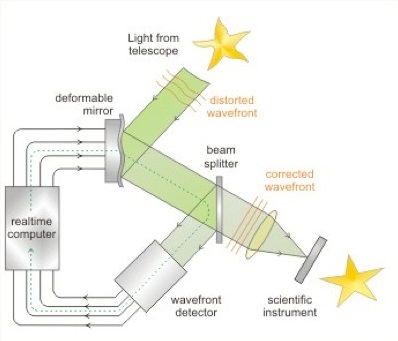
\includegraphics[width=0.6\textwidth,angle=0]{Figures/ao_scheme.jpg}
\caption{Adaptive optics schema}
source : Institut National of Astrophysics, Bologna Observatory, 2018, \url{http://www.bo.astro.it/ter5/ter5/ao.html}.
\label{fig:ao_scheme}
\end{center}
\end{figure}

In the 1980's, systems to correct aberrations in telescopes called an active optics system were developed. It consists of actuators placed under the telescope mirrors capable of correcting the telescope deformation due to the effect of wind, temperature, gravity, vibration, etc... Those systems works at  around 1 Hz , which is not fast enough to correct for the turbulence of the atmosphere (100-1000 Hz) but they are essential in the construction of large telescopes. The state-of-the-art technique is the adaptive optics, developed to take into account the effects of the atmosphere. This technique monitors the aberrations present in the wavefront and corrects them in real time. The schema of principle is shown in Figure \ref{fig:ao_scheme}. It uses a wavefront sensor to characterize its deformation and then passes the information to a deformable mirror to correct it. It is called an adaptive optic loop. It works well, but the drawback of this method is that it does not correct the aberrations up to the scientific detector. Those uncorrected aberrations are called Non-Common Path Aberration (NCPA), they are generally static or slowly evolving over time. The adaptive optic also requires a complex optical system before the scientific detector. The beam is split in two parts. One arm goes to the scientific detector and the other is used in the adaptive optic loop.

We present here a method called phase diversity that uses images of the scientific detector to deduct the aberrations present in the wavefront. In our case, the phase diversity is used to correct the static aberrations that deform the wavefront. Our work is inspired by the phase diversity idea that was first introduced by \citet{Gonsalves_1982}. The idea is to use one focused and one defocused image to retrieve the aberrations. Two images at least are needed due to the property of light acquisition. There is an indetermination, because the detector is only sensitive to the intensity of light and not the light wave itself. This indetermination is raised adding a phase diversity. Unlike adaptive optic system, the phase diversity requires nearly no additional optical component depending on how it is implemented. The final aim of this project would be to integrate the developed phase diversity into the design of the DAG (Dogu Anadolu Gozlemevi) telescope in Turkey, see Figure \ref{fig:DAGtelescope}.

\begin{figure}
\begin{center}
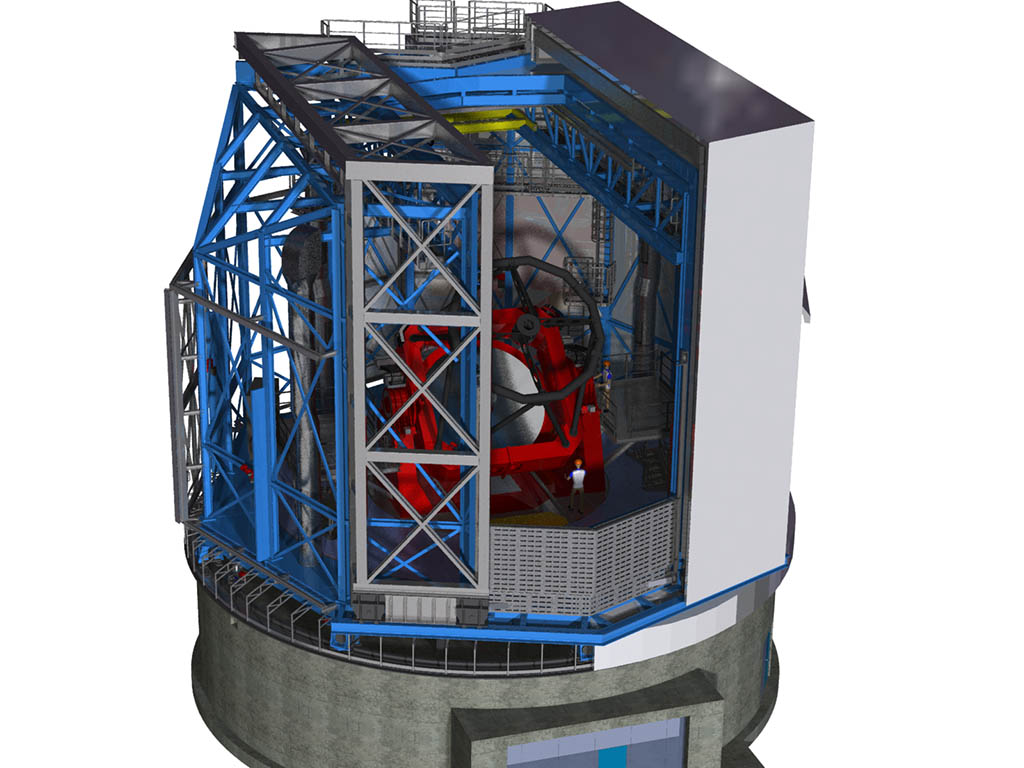
\includegraphics[width=0.5\textwidth,angle=0]{Figures/DAGtelescope.jpg} \\
\caption{DAG 4m telescope} 
source : EIE group, 2018, \url{http://www.eie.it/en/progetti/dag-dogu-anadolu-gozlemevi}.
\label{fig:DAGtelescope}
\end{center}
\end{figure}

\vspace{1cm}

This report is organized in three main chapters. First, a review of the necessary theoretical background is reminded, going from the scalar theory of diffraction to the description of phase retrievals methods. Then we present an experiment performed at the optic laboratory at HEIG-VD. The ONERA (Office National d'Etudes et de Recherches Aerospatiales) algorithm of phase diversity is tested and used in comparison with a Shack-Hartmann wavefront sensor. And finally, the development of an analytical phase diversity algorithm is presented and tested with simulated Point Spread Functions (PSFs).

\chapter{Theoretical background} 
\label{ch:THback}

In this chapter, the basic theory of our work is presented. First, the light propagation formalism is reminded through the scalar diffraction theory based on the book written by \citet{goodman_1968}. Then the general properties of an imaging system are described. And finally we present the wavefront aberration theory and two different methods to identify and correct the aberrations.

\section{Scalar Diffraction Theory}
\label{sec:ScaDifTh}

\subsection{Scalar Field and Helmholtz equation}
\label{subsec:ScalF_HelmEqt}

A monochromatic wave, at position $P$ and time $t$, can be represented by a scalar field $u(P,t)$ written as :

\begin{equation}
u(P,t) =  A(P) exp\left[-j2\pi\nu t - j\phi(P)\right],
\label{eqt:WvscalarField}
\end{equation}

where $A(P)$ and $\phi(P)$ are the amplitude and phase, respectively, of the wave at position P and $\nu$ is the wave frequency.

The spatial part of eqt. \eqref{eqt:WvscalarField}, also called  phasor  in the literature, 

\begin{equation}
U(P) = A(P)e^{-j\phi(P)},
\label{eqt:phasor}
\end{equation}

must verify the Helmotz equation : 

\begin{equation}
(\nabla^2 + k^2)U = 0,
\label{eqt:HelmholtzEqt}
\end{equation}

where $k$ is the wave number given by

\begin{equation}
k = 2\pi n \frac{\nu}{c} = \frac{2\pi}{\lambda},
\label{eqt:wavenumber}
\end{equation}

and $\lambda$ is the wavelength in the dielectric medium.


\subsection{Rayleigh-Sommerfeld integral}
\label{subsec:Ray_Som_int}

\begin{figure}
\centering
    \begin{subfigure}{0.4\textwidth}
        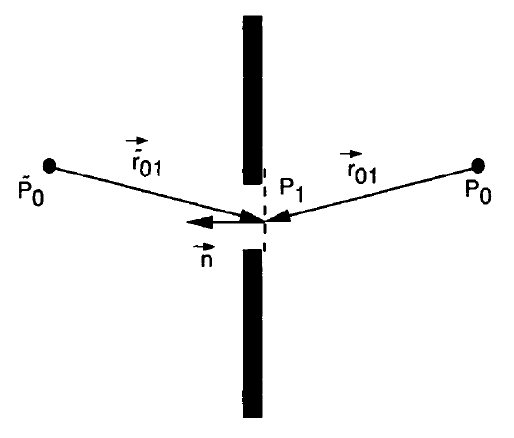
\includegraphics[width=\textwidth]{Figures/Ray_Som_Diff}
        \caption{Rayleigh-Sommerfeld formulation of diffraction by a plane screen, \citep[Chapter 3.5]{goodman_1968}.}
        \label{subfig:Ray_Som_Diff}
    \end{subfigure}
    \quad
    \begin{subfigure}{0.5\textwidth}
        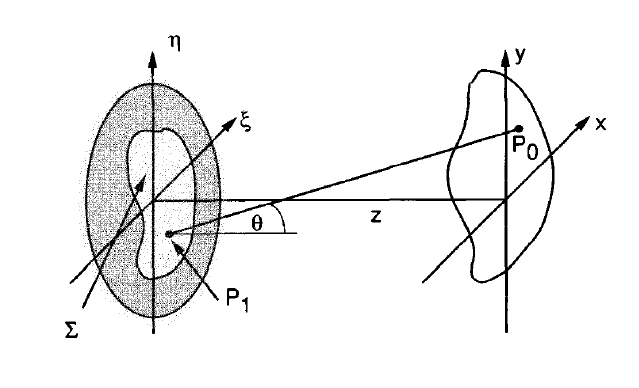
\includegraphics[width=\textwidth]{Figures/Diff_Geom}
        \caption{Diffraction geometry, \citep[Chapter 4.1]{goodman_1968}.}
        \label{subfig:Diff_Geom}
    \end{subfigure}
    \decoRule
    \caption{Diffraction Schemas}
    \label{fig:Diff_Schemas}
\end{figure}

Rayleigh and Sommerfeld developed a formalism using the Helmholtz equation and Green's Theorem to compute the induced diffraction by a plane screen. Let's suppose that we have a monochromatic source at $\widetilde{P_0}$ on the left of a plane screen with aperture $\Sigma$, the Rayleigh-Sommerfeld formula allows to compute the complex amplitude at $P_0$ on the right of the plane screen (see Figure \ref{subfig:Ray_Som_Diff}).

\begin{equation}
U(P_0) = \frac{1}{j\lambda} \iint\limits_{\Sigma} U'(P_1)\frac{exp(jkr_{01})}{r_{01}}cos(\mathbf{n},\mathbf{r_{01}})\mathbf{ds}
\label{eqt:Ray_Som_Formula}
\end{equation}

$U'(P_1)$ is the wave field on the screen and $cos(\mathbf{n},\mathbf{r_{01}})$ is the cosine of the angle between the aperture plane normal toward the source and the vector $\mathbf{r_{01}} = \mathbf{P_0P_1}$ given by 

\begin{equation}
r_{01} = \sqrt{z^2 + (x-\xi)^2 + (y-\eta)^2}.
\label{eqt:r_01}
\end{equation}

We can rewrite eqt. \eqref{eqt:Ray_Som_Formula} using $cos(\mathbf{n},\mathbf{r_{01}}) = cos(\theta) = \frac{z}{r_{01}}$ and the coordinate systems ($\xi,\eta$) and ($x,y$), see Figure \ref{subfig:Diff_Geom},

\begin{equation}
U(x,y) = \frac{z}{j\lambda} \iint\limits_{-\infty}^{\infty} U(\xi,\eta)\frac{exp(jkr_{01})}{r_{01}^2} d\xi d\eta.
\label{eqt:Ray_Som_formula_xy_en}
\end{equation}

We can integrate from $-\infty$ to $\infty$, using $U(\xi,\eta) = P(\xi,\eta)U'(\xi,\eta)$ where $P(\xi,\eta)$ is the pupil function. The latter equals to one in the pupil and zero outside. 

\subsection{Fresnel approximation}
\label{subsec:FresnelApprox}

To reduce eqt. \eqref{eqt:Ray_Som_formula_xy_en}, also known as the Huygens-Fresnel principle, one can approximate the distance $r_{01}$ using the taylor expansion of the square root :

\begin{equation}
r_{01} = z \sqrt{1 + \frac{x-\xi}{z} + \frac{y-\eta}{z}} \approx z \left[1+\frac{1}{2}\left(\frac{x-\xi}{z}\right)^2+\frac{1}{2}\left(\frac{y-\eta}{z}\right)^2\right]
\label{eqt:approx_r01}
\end{equation}

To obtain the Fresnel approximation, one has to replace $r_{01}$ by eqt. \eqref{eqt:approx_r01} in eqt. \eqref{eqt:Ray_Som_formula_xy_en}. At the denominator, only the first term $z$ is kept, since the introduced error is small. But in the exponential everything is kept. Then the final expression is given by,

\begin{equation}
U(x,y) = \frac{e^{jkz}}{j\lambda z} \iint\limits_{-\infty}^{\infty} U(\xi,\eta)exp \left\lbrace j \frac{k}{2z}\left[(x-\xi)^2+(y-\eta)^2\right]\right\rbrace d\xi d\eta.
\label{eqt:fresnel_Approx_conv}
\end{equation}

In this form, the Fresnel approximation can be seen as a convolution between $U(\xi,\eta)$ and $h(x,y) = \frac{e^{jkz}}{j\lambda z}exp\left[\frac{jk}{2z}\left(x^2+y^2\right)\right]$.

Another form is found by developing $\left[(x-\xi)^2+(y-\eta)^2\right]$,

\begin{equation}
U(x,y) = \frac{e^{jkz}}{j\lambda z} e^{j\frac{k}{2z}(x^2+y^2)} \iint\limits_{-\infty}^{\infty} \left\lbrace U(\xi,\eta) e^{j\frac{k}{2z}(\xi^2+\eta^2)}\right\rbrace e^{-j\frac{2\pi}{\lambda z}(x\xi+y\eta)} d\xi d\eta,
\label{eqt:fresnel_Approx_FT}
\end{equation}

this is the Fourier transform of the complex field in the pupil multiplied by a quadratic phase exponential.

\subsection{Fraunhofer approximation}
\label{subsec:FraunhoferApprox}

In addition to the Fresnel approximation, we can introduce another approximation using the condition,

\begin{equation}
z >> \frac{k(\xi^2+\eta^2)_{max}}{2}.
\label{eqt:Fraun_Cond}
\end{equation}

If eqt. \eqref{eqt:Fraun_Cond} is satisfied the Fresnel approximation simplifies, since the quadratic phase factor in $(\xi,\eta)$ is approximately one on the entire pupil, as

\begin{equation}
U(x,y) = \frac{e^{jkz}}{j\lambda z} e^{j\frac{k}{2z}(x^2+y^2)} \iint\limits_{-\infty}^{\infty} U(\xi,\eta) e^{-j\frac{2\pi}{\lambda z}(x\xi+y\eta)} d\xi d\eta.
\label{eqt:Fraunhofer_approx}  
\end{equation}

For instance, at a wavelength of 637.5 nm and a pupil diameter of 3.6 mm the Fraunhofer approximation constrains $z$ to be greater than 63 meters to be valid.

\subsection{Converging lens introduction}
\label{subsec:ConvLensIntro}

The Fraunhofer conditions are severe as shown above, but one can reduce the distance $z$ by observing the focal plane of a converging lens. Indeed, using the paraxial approximation, i.e. small angles with respect to the optical axis, the lens transmission function is given by,

\begin{align}
t_l(\xi , \eta) &= exp \left[ j k n \Delta_0 \right] exp \left[ -jk \left( n-1 \right)\frac{ \xi^2 + \eta^2 }{2}\left( \frac{1}{R_1} - \frac{1}{R_2}\right) \right] \nonumber \\ 
&= exp \left[ -j \frac{k}{2f} (\xi^2+\eta^2) \right] ,
\label{eqt:lensTl}
\end{align}

where $n$ is the refractive index of the lens material, $R_1$ and $R_2$ are the curvature's radii of the front and back surface of the lens, respectively, and f is the lens focal length defined as,

\begin{equation}
\frac{1}{f} \equiv (n-1)\left(\frac{1}{R_1}-\frac{1}{R_2}. \right)
\label{eqt:focal_length}
\end{equation}

We can define $U_l(\xi,\eta) = U(\xi,\eta)t_l(\xi,\eta)$, which represents the complex amplitude passing through a lens. Finally, replacing $U(\xi,\eta)$ by $U_l(\xi,\eta)$ in Fresnel approximation and setting the observing distance to the focal length of the converging lens, we recover the Fraunhofer approximation,

\begin{align}
U(x,y) &= \frac{e^{jkz}}{j\lambda z} e^{j\frac{k}{2z}(x^2+y^2)}  \mathcal{F}\left\lbrace U(\xi,\eta) exp\left[j\frac{k}{2}(\xi^2+\eta^2)(\frac{1}{z}-\frac{1}{f})\right]\right\rbrace \nonumber \\
&\overset{z=f}{=} \frac{e^{jkz}}{j\lambda z} e^{j\frac{k}{2z}(x^2+y^2)}  \mathcal{F}\left\lbrace U(\xi,\eta)\right\rbrace.
\end{align}

\section{Imaging system}
\label{sec:ImSystem}

\begin{figure}
\begin{center}
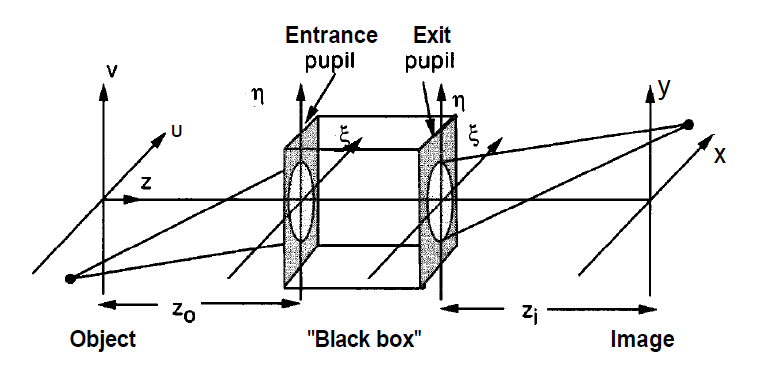
\includegraphics[width=0.8\textwidth,angle=0]{Figures/ImagingInstrumentGenSchema}
\decoRule
\caption{Schema of a imaging instrument, \citep[Chapter 6.1]{goodman_1968}}
\label{fig:ImagingInstrumentGenSchema}
\end{center}
\end{figure}

An imaging system, such as a telescope, is used to acquire images of an object as perfectly as possible, generally working with high magnification to observe far object with details. An optical system, forming an instrument, is composed by lenses, mirrors, etc... and a detector (can be the human eye). A complex optical system can be reduced to a pupil, $P(\xi,\eta)$, and a focal length, $f$. The diffraction of the wave can be determined by the Fraunhofer approximation as long as the paraxial approximation is valid, see subsection \ref{subsec:ConvLensIntro}. And the observed image of an incoherent object at the system's focal plane is proportional to the square modulus of the phasor $U(x,y)$,

%\begin{equation}
%i(x,y) \alpha |\left[\mathcal{F}\left\lbrace U(\xi,\eta) \right\rbrace\right](x,y)|^2.
%\label{eqt:i_modu_FT}
%\end{equation}

\subsection{Impulse Response (IR)}
\label{subsec:IR} 

\begin{figure}
\centering
    \begin{subfigure}{0.45\textwidth}
        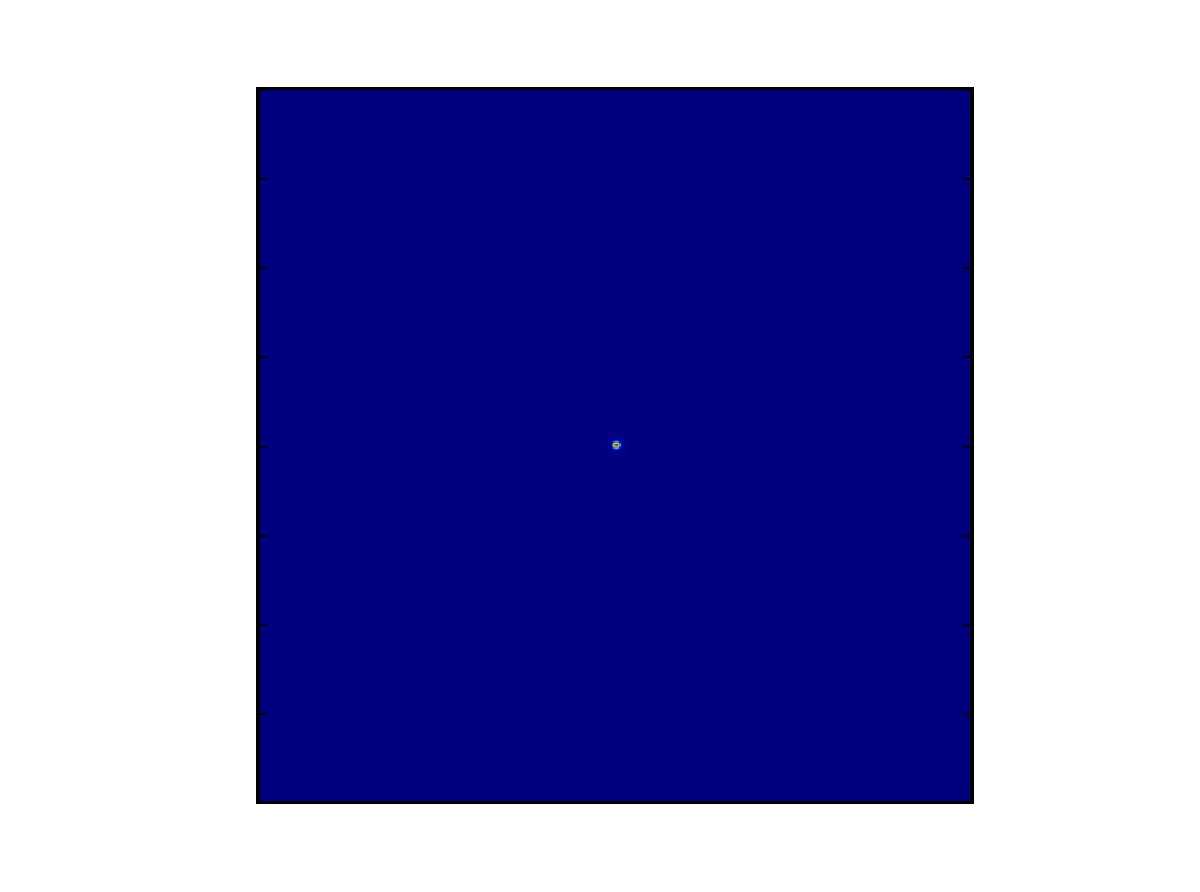
\includegraphics[width=\textwidth]{Figures/PSF}
        \caption{PSF}
        \label{subfig:PSF}
    \end{subfigure}
    \quad
    \begin{subfigure}{0.45\textwidth}
        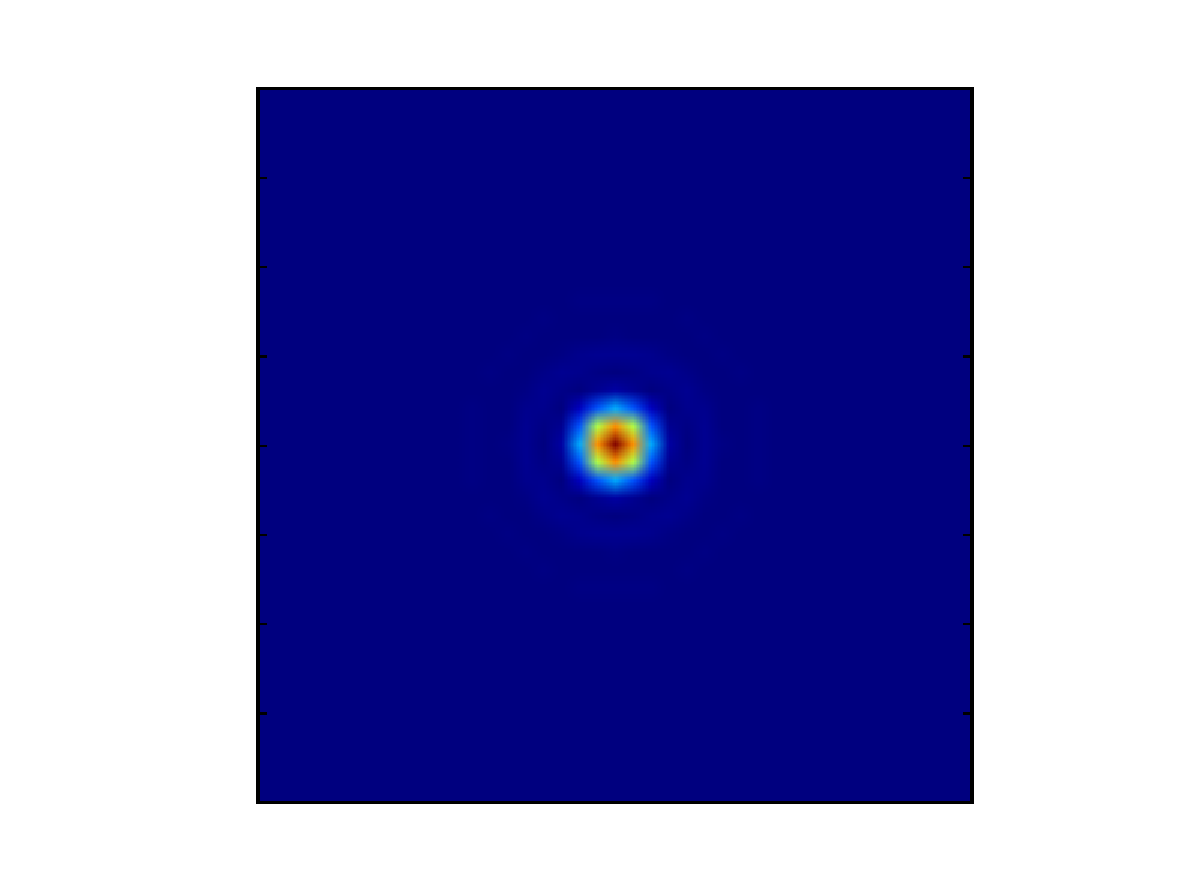
\includegraphics[width=\textwidth]{Figures/PSFzoom}
        \caption{PSF zoom x10}
        \label{subfig:PSFzoom}
    \end{subfigure}
    \decoRule
    \caption{PSF of a perfect imaging system composed by a 3.6 mm pupil and a focal length of 80 mm at a wavelength of 637.5 nm. The size, N, of the PSF is 400 pixels and the pixel size is 5.3 $\mu m$.}
    \label{fig:PSF}
\end{figure}

The impulse response or PSF, $h(x,y;u,v)$, of an optical system is  the field amplitude induced at coordinates $(x,y)$ by a unit-amplitude point source at object coordinates $(u,v)$. An example of PSF for a incoherent point source object is shown in Figure \ref{fig:PSF}. Using the linearity of the wave propagation, we can write the imaged amplitude as a superposition integral,

\begin{equation}
U(x,y) = \iint_{-\infty}^{\infty} h(x,y;u,v)U(u,v)dudv.
\label{eqt:superpositionIntegral}
\end{equation}

\subsection{Optical Transfer Function (OTF)}
\label{subsec:OTF}

\begin{figure}
\begin{center}
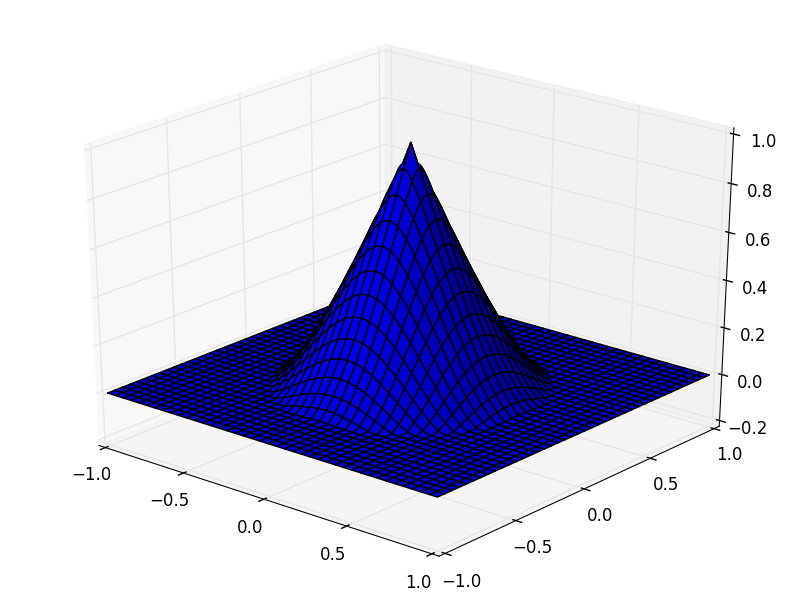
\includegraphics[width=0.5\textwidth,angle=0]{Figures/OTF}
\decoRule
\caption{OTF of a perfect imaging system composed by a 3.6 mm pupil and a focal length of 80 mm at a wavelength of 637.5 nm.}
\label{fig:OTF}
\end{center}
\end{figure}

The optical transfer function, OTF, is defined as the Fourier transform of the impulse response,

\begin{equation}
\widetilde{h}_{optical}(\xi,\eta) = \mathcal{F}\left\lbrace h_{optical}(x,y)\right\rbrace ,
\label{eqt:OTF}
\end{equation}

where $\xi$ and $\eta$ are the conjugate variables of $x$ and $y$ with respect to the Fourier transform.

An example for an incoherent point source is shown in Figure \ref{fig:OTF} and it correspond to the OTF of the PSF shown in Figure \ref{fig:PSF}. For incoherent illumination, using the Fourier transform properties it can also be given by the autocorrelation of the pupil function as we will see in section \ref{subsec:FromOtoI},

\begin{equation}
\widetilde{h}_{optical}(\xi,\eta) = (P \otimes P)(\xi,\eta).
\label{eqt:}
\end{equation}


\subsection{Image formation}
\label{subsec:FromOtoI}

A detector only senses the energy distribution produced by an electromagnetic wave. Therefore, an image is given by the square modulus of the complex amplitude at the focal plane,

\begin{equation}
i(x,y) = |U(x,y)|^2 = |\iint_{-\infty}^{\infty} h(x,y;u,v)U(u,v)dudv|^2.
\label{eqt:IsqAmplitude}
\end{equation}

This integral simplifies differently depending on the type of object we are observing. 

For a \textbf{coherent object}, \citet[Chapter 6.2]{goodman_1968} showed that the imaging is linear in complex amplitude, thus eqt. \eqref{eqt:IsqAmplitude} becomes,

\begin{equation}
i(x,y) = |\iint_{-\infty}^{\infty} h(x-\widetilde{u},y-\widetilde{v})U(\widetilde{u},\widetilde{v})d\widetilde{u}d\widetilde{v}|^2,
\label{eqt:convolution_hUo}
\end{equation}

where $(\widetilde{u} = Mu,\widetilde{v}= Mv)$ are the normalized object coordinates and $M$ is the magnification of the imaging system. The image is given by the squared modulus of the convolution of the impulse response and the object complex amplitude.

For an \textbf{incoherent object},  \citet[Chapter 6.2]{goodman_1968} showed that the imaging is linear in intensity,

\begin{equation}
i(x,y) = \iint_{-\infty}^{\infty}|h(x-\widetilde{u},y-\widetilde{v})|^2o(\widetilde{u},\widetilde{v})d\widetilde{u}d\widetilde{v} = (h_{optical}\otimes o)(x,y),
\label{eqt:imageObjectrel}
\end{equation}

where $o(x,y) = |U(x,y)|^2$. We can recognize the convolution of an object with an intensity impulse response, $h_{optical}(x,y) = |h(x,y)|^2$.

In this thesis, we study star-like radiation which are object with an incoherent emission. Stars are point source objects given their distances. The image that an optical system gives of a point source is called the point spread function, PSF, or impulse response, IR, of the system, see Figure \ref{fig:PSF}. A point source is characterized by an infinite distance to the instrument and therefore the wave is planar, which means that the phasor is reduced to $U(\xi,\eta) = P(\xi,\eta)$. The PSF or IR is given by,

\begin{equation}
h_{optical}(x,y) = |\left[\mathcal{F}\left\lbrace P(\xi,\eta) \right\rbrace\right](x,y)|^2
\label{eqt:impulseResponse}
\end{equation}

The domain where the impulse response is invariant under translation is called the \textbf{isoplanatic domain}.

In presence of aberrations, which will be discussed in section \ref{sec:Aberrations}, the wavefront is deformed with respect to the perfect planar or spheric form. The pupil function at the exit of the imaging system is modified as following,

\begin{equation}
\mathcal{P}(\xi,\eta) = P(\xi,\eta) e^{-j\phi_{Ab}(\xi,\eta)},
\label{eqt:aberratedPhasor}
\end{equation}

where $\phi_{Ab}(\xi,\eta)$ is the dephasing caused by the aberrations present between the object and the image planes. Replacing the new pupil function in eqt. \eqref{eqt:impulseResponse}, we obtain the PSF of an imaging system having aberrations on the optical path.

\section{Aberrations}
\label{sec:Aberrations}

\begin{minipage}{\linewidth}
\begin{wrapfigure}{r}{0.5\textwidth}
\centering
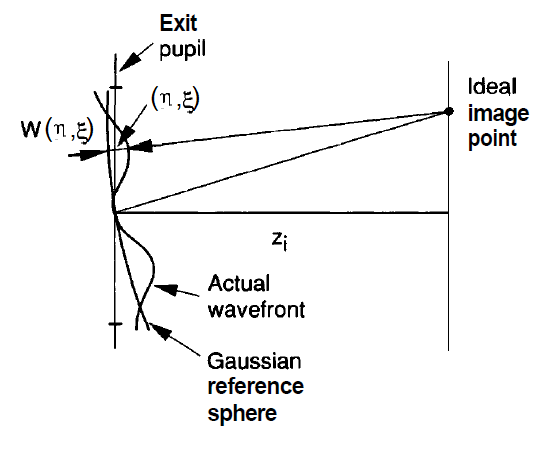
\includegraphics[width=0.5\textwidth]{Figures/AbWFvsGausSphWF}
\decoRulewrapFig
\caption[Gaussian reference sphere vs. aberrated Wavefront]{Gaussian reference sphere vs. aberrated Wavefront, \citep[Chapter 6.4]{goodman_1968}. The dephasing is equal to the wave number multiplied by the aberration function, $\phi_{Ab}(\xi,\eta) = k W(\xi,\eta)$.}
\label{fig:AbWFvsGausSphWF}
\end{wrapfigure}

The aberrations present on the optical path between the object and the image plane decrease the quality of the resulting image. Indeed, they induce fluctuations of the amplitude and phase of the wave in the pupil plane. Since the amplitude fluctuations are negligible with respect to the phase fluctuations, we focus only on the latter. In figure \ref{fig:AbWFvsGausSphWF}, one can see the aberration's effect on an hypothetical spherical wavefront at the exit pupil of an imaging system. And in Figure \ref{fig:ComparisonPSFs}, one can see the effect of aberrations on the PSF of an imaging system. The PSF is blurred due to the defocus and we can well recognize the astigmatism introduced as the PSF's shape tends towards an ellipse. The Strehl ratio is often used to quantify the importance of the aberrations, it is given by the following expression,

\begin{equation}
SR = \frac{\int \widetilde{h}_{optical}(\xi,\eta)\mathrm{d}\xi \mathrm{d}\eta}{\int \widetilde{h}_{perfect}(\xi,\eta) \mathrm{d}\xi \mathrm{d}\eta},
\label{eqt:StrehlRatio}
\end{equation}

where $\widetilde{h}_{perfect}(\xi,\eta)$ is the OTF of the perfect system with the same pupil as the optical system with the OTF $\overset{\sim}{h}_{optical}(\xi,\eta)$.
\end{minipage}

\begin{figure}
 \centering
     \begin{subfigure}{0.45\textwidth}
         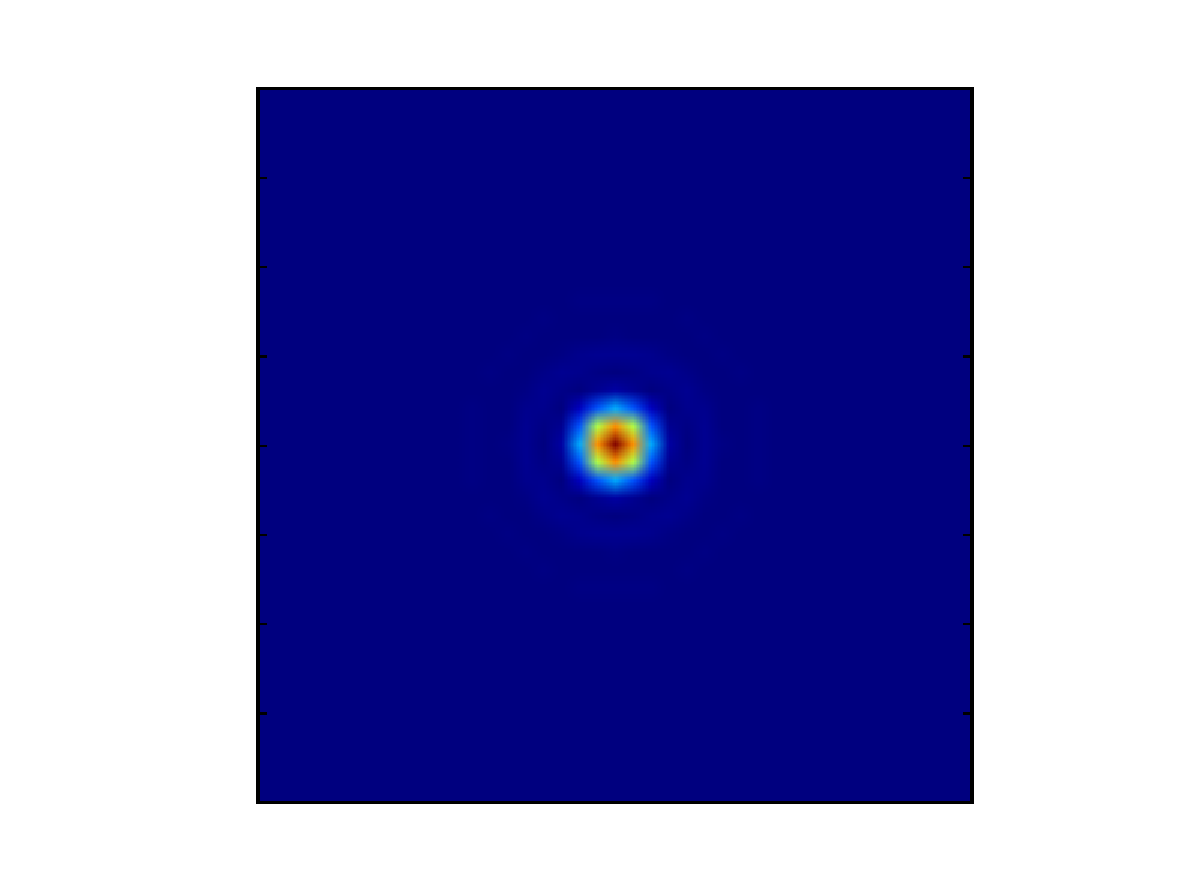
\includegraphics[width=\textwidth]{Figures/PSFzoom}
         \caption{perfect PSF (zoomed x10)}
         \label{subfig:perfPSF}
     \end{subfigure}
     \quad
     \begin{subfigure}{0.45\textwidth}
         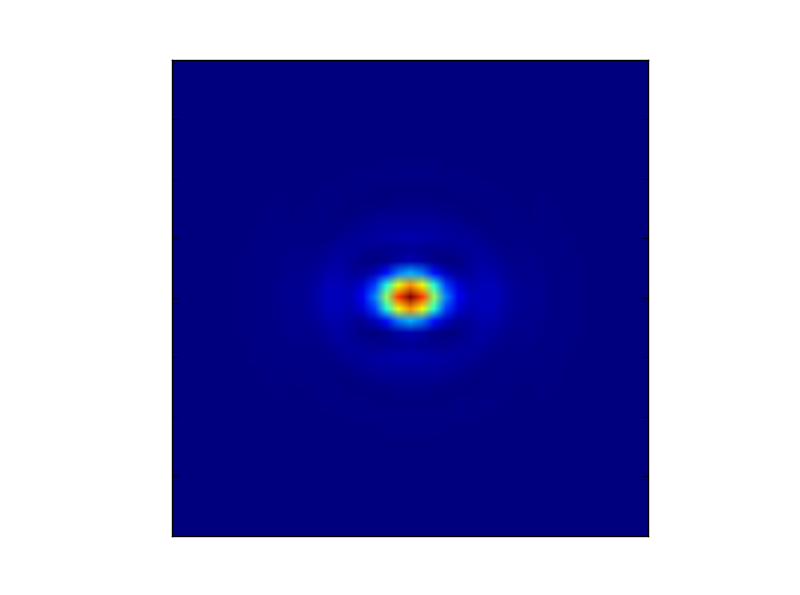
\includegraphics[width=\textwidth]{Figures/PSFzoomWthAb}
         \caption{PSF with aberrations (The Zernike coefficients are $a_j = 50 \mathrm{nm}$ for $a_{4}$, $a_{6}$and $a_{11}$, see subsec \ref{subsec:ZernikePol} for the definition of $a_j$, zoomed x10)}
         \label{subfig:PSFWthAb}
     \end{subfigure}
     \decoRule
     \caption{Comparison of perfect PSF and PSF with aberrations of an imaging system composed by a 3.6 mm pupil and a focal length of 80 mm at a wavelength of 637.5 nm. The size, N, of the PSF is 400 pixels and the pixel size is 5.3 $\mu m$.}
     \label{fig:ComparisonPSFs}
 \end{figure} 

\subsection{Sources of aberration}
\label{subsec:SourcesAb}

The phase fluctuations introduced by aberrations are due to different kind of perturbations on the optical path. In ground based astronomy, the main source of aberrations is the \textbf{atmosphere}. Indeed, the atmosphere's temperatures fluctuations coupled with turbulent airflows are at the origin of the refractive index's variations. Those variations induce different optical paths, in other words they generate perturbations on an electromagnetic wave passing through the atmosphere. The theory of the Atmospheric Turbulence is beyond the scope of this work, but we redirect the interested reader to \citet{obukhov1949,Tatarski1961,kolmogorov1968}.

The other source of aberrations are the \textbf{defects of the instrument} itself. The flaws can limit the resolution and decrease the quality of a diffraction-limited imaging system. The defects can have multiple origins as described by \citet{Blanc2002}. The first one is a \textbf{defect during the fabrication process}, such as mirror polishing. This kind of defect is constant over time and of high spatial frequency. Perturbation of the electromagnetic wave can also be due to \textbf{misalignment of the optical instrument's components}. For instance, during the first stages of operation of the Hubble telescope, the mirrors were not correctly aligned and the resulting images were blurry. These defects are of low spatial frequencies and vary slowly over time. Finally, there are defects due to \textbf{mechanical stresses of the instrument}. The mirrors have to be held in place by different mechanical components. And under the influence of the gravity, a mirror deformation can arise resulting in an aberrations introduction. This kind of defect also evolves slowly through time but has a large spatial frequency domain.

We focus on a method to correct the effects of the instrument flaws. The method is particularly suited since it does not require a different path than the path to the scientific instrument, which means that we can correct the aberrations on the entire optical path.

\subsection{Zernike polynomials}
\label{subsec:ZernikePol}

\begin{figure}
\begin{center}
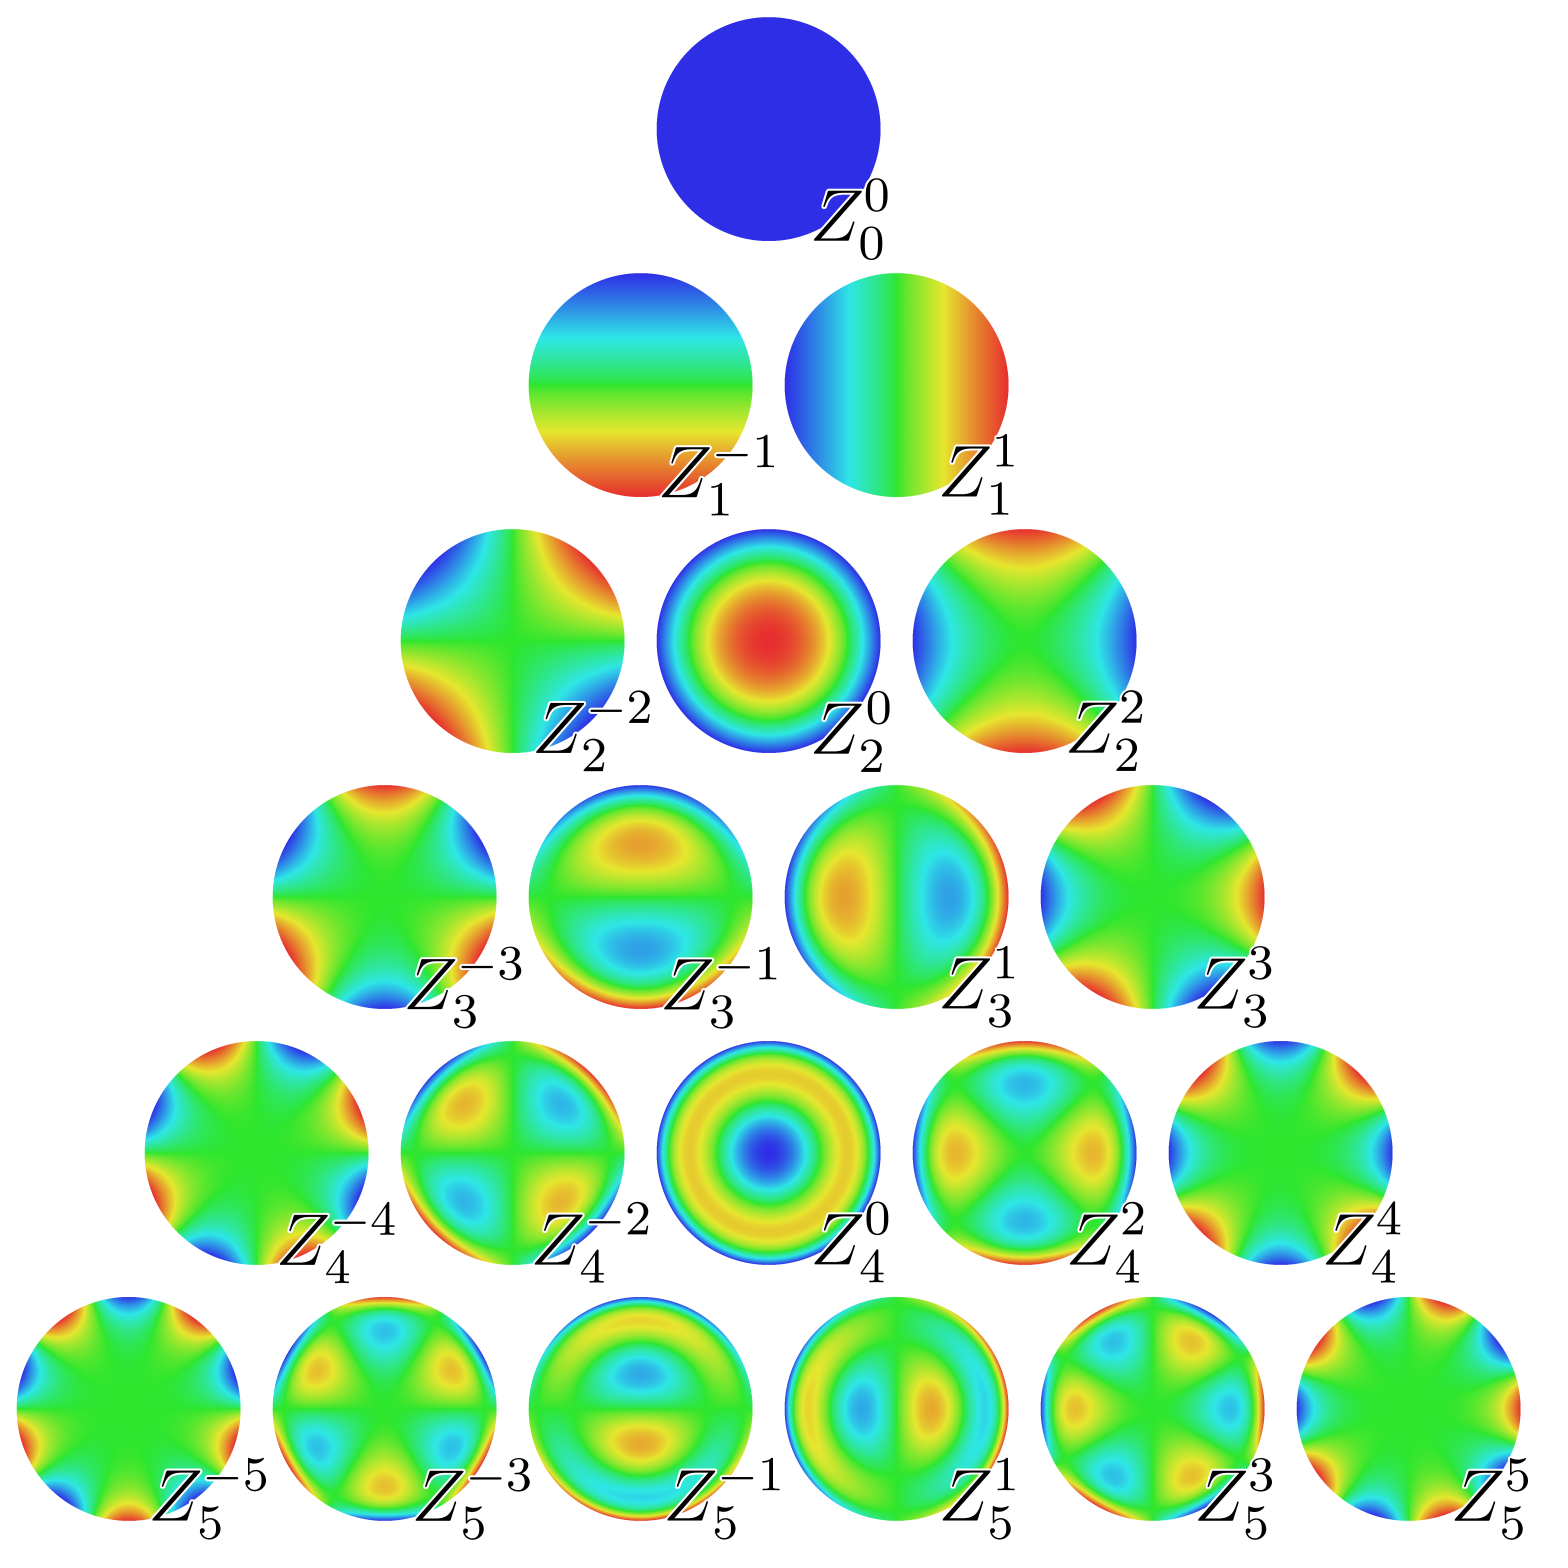
\includegraphics[width=\textwidth,angle=0]{Figures/Zernike_polynomials}
\decoRule
\caption[Representation of the 21 first Zernike polynomials]{Representation of the 21$^{st}$ Zernike polynomials \citep{ZernikeWiki}}
\label{fig:Zernike_polynomials}
\end{center}
\end{figure}


In order to study the aberrations present in an imaging system, \citet{zernike1934} introduced an orthonormal basis on which we can decompose the phase on a circular pupil, such as a telescope pupil. Those polynomials are the product of a trigonometric function and a radial polynomial function \citep{Noll_1976}.

\begin{equation}
Z_j(\mathbf{r}) = R_n^m(r)\Theta^m_n(\theta),
\label{eqt:ZernikePol}
\end{equation}

where $r=\frac{r'}{R_{pup}}$ is the normalized radius on the unit circle and $\theta$ is the azimuthal angle on the unit circle. $j$ correspond to the Zernike index in the Noll order, a specific $j$ corresponds only to one couple $(n,m)$. The values of n and m satisfy the conditions $|m| \leq n$ and $n - |m| = \mathrm{even}$.

The trigonometric function is given by,

\begin{equation}
\Theta_n^m(\theta) = 
\begin{cases} 
\sqrt{n+1} &if m=0, \\
\sqrt{2(n+1)}cos(m\theta) &\mathrm{if} \ m \neq 0 \ \mathrm{and} \ i \ \mathrm{even}, \\
\sqrt{2(n+1)}sin(m\theta) &\mathrm{if} \ m \neq 0 \ \mathrm{and} \ i \ \mathrm{odd},
\end{cases}
\label{eqt:trigoFunc}
\end{equation}

and the radial function is given by,

\begin{equation}
R_n^m(r) = \sum\limits_{s=0}^{(n-m)/2}\frac{(-1)^s(n-s)!}{s![(n+m)/2-s]![(n-m)/2-s]!}r^{n-2s}.
\label{eqt:radialFunction}
\end{equation}

The decomposition of the phase onto the Zernike polynomials is given by,

\begin{equation}
\phi (\mathbf{r}) = \sum\limits_{i=1}^{+\infty}a_iZ_i(\mathbf{r}),
\label{eqt:decompPhase}
\end{equation}

where the $a_i$'s are the Zernike coefficients. And we characterize a wavefront by its root mean squared error (RMS error or RMSE) which is given by,

\begin{equation}
\sigma_{\phi} = \sqrt{\frac{1}{S}\int\limits_S \phi^2(\mathbf{r})d\mathbf{r}} = \sqrt{\sum\limits_{i=2}^{+\infty}a_i^2},
\label{eqt:WFrmsError}
\end{equation}

where $S$ is the surface of the pupil.

\section{Phase retrieval}

The phase retrieval is a complicated process since the detectors are only sensitive to the intensity of a wave and not the wave itself, which prevents us to obtain a direct relation between phase and image. Thus, we only have an indirect measurement of the wavefront. Nevertheless, it is important to be able to estimate the aberrations of a system in order to correct them in real-time (Adaptive Optics systems) or in post-processing (Image restoration).

There are a couple of ways to characterize the form of a wavefront, i.e. to determine the amplitude of the aberrations present in an imaging system. Some uses the optical geometric approximation, which says that locally the light rays are perpendicular to the wavefront. These achromatic methods measure the gradient of the wave surface, such as Shack-Hartmann \citep{hartmann1900,ShackPlatt_1971,fontanella1985}, Curvature sensing \citep{Roddier1988} and Pyramid sensing \citep{ragazzoni1996}. Another kind of methods is called interferometric or focal plane methods. They use the interference patterns of the pupil to determine the form of the wavefront. The \textbf{Phase Diversity} is part of those kind of methods. It was first proposed by \citet{Gonsalves_1982}. The most popular methods nowadays are the Shack-Hartmann, the curvature sensing and the phase diversity. We explain the principle of a Shack-Hartmann sensor and phase diversity in the two next subsections.


\subsection[Shack-Hartmann]{Shack-Hartmann \citep{hartmann1900,ShackPlatt_1971}}
\label{subsec:SHprinciple}

\begin{figure}
\begin{center}
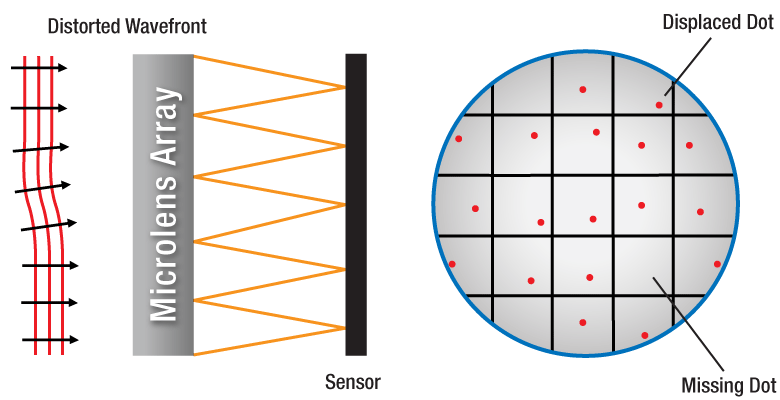
\includegraphics[width=\textwidth,angle=0]{Figures/SHWFSPrinciple}
\decoRule
\caption[Shack-Hartmann principle]{Shack-Hartmann principle \citep{SHWFS}}
\label{fig:SHWFSPrinciple}
\end{center}
\end{figure}

The Shack-Hartmann wavefront sensor measures the gradient of an aberrant phase. Figure \ref{fig:SHWFSPrinciple} shows the principle. A micro-lenses array samples the wavefront passing through the pupil in a conjugated plane of the entrance pupil. Each micro-lens produces a dot on a CCD placed at the foci of the micro-lenses. The deformations of the wavefront induce a displacement of the dot with respect to a reference position obtained with a perfectly planar or spherical wavefront. By measuring these displacements, $\Delta x$ and $\Delta y$, it gives directly the local slope of the wavefront \citep{fontanella1985},

\begin{equation}
\frac{2\pi}{\lambda}\frac{\Delta s}{f} = \frac{1}{S} \iint\limits_S \frac{\delta\phi (x,y)}{\delta s}dxdy,
\label{eqt:SHWFSlope}
\end{equation}

where $s$ is either $x$ or $y$ and S is the surface of a micro-lens and f is the focal length of the micro-lenses. The wavefront is reconstructed by integrating over all the local slope measurements. The advantage of this technique is that it does not require a lot of computation since it is a direct measurement. But it requires an important optical system to acquire the data. It is used in many fields, especially in adaptive optics systems to correct the atmospheric turbulence.

\subsection{Phase Diversity}
\label{subsec:PDprinciple}

The phase diversity was first implemented by R. A. Gonsalves in 1976 \citep{Gonsalves_1976,Gonsalves_1982} to retrieve the phase of a wavefront coming from a point source. It uses two images, one at the focal plane and another one with a diversity introduced, such as a defocus, in order to recover the phase of the wavefront.

\begin{figure}
\begin{center}
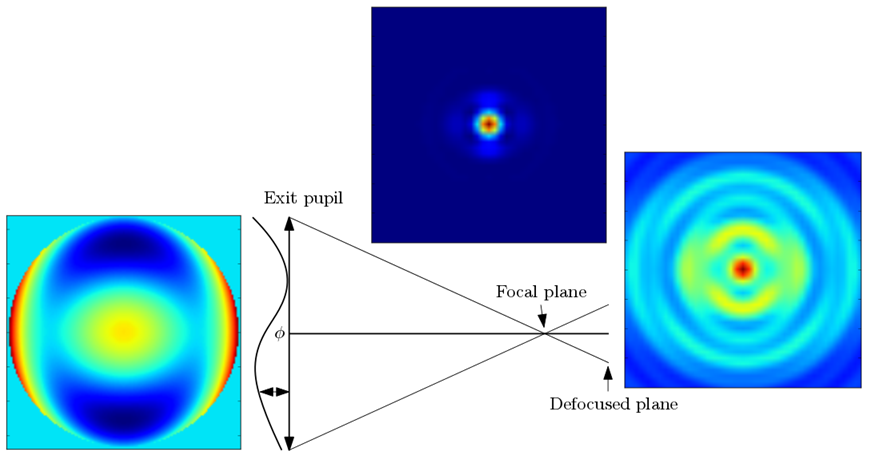
\includegraphics[width=0.8\textwidth,angle=0]{Figures/DiversityPrincipleM}
\decoRule
\caption{Schema of the phase diversity principle. The images from left to right are : the phase arriving on the exit pupil, the focused image and the defocused ($2\pi$) image.}
\label{fig:DiversityPrinciple}
\end{center}
\end{figure}

Unlike Shack-Hartmann wavefront reconstruction, which is a pupil plane technique, the phase diversity uses data acquired at the focal plane. Using the non-linear relation between the phase of the wavefront and the image, 

\begin{equation}
i(x,y) = (h_{optical}\otimes o)(x,y), \ with \ h_{optical}(x,y) = |\left[\mathcal{F}\left\lbrace A(\xi,\eta)e^{j\phi(\xi,\eta)} \right\rbrace\right](x,y)|^2,
\label{eqt:img-hopt}
\end{equation}

one can determine the phase, i.e. the aberrations present in the imaging system, by solving an inverse problem. The major difficulty of this technique is that, as one can see in eqt. \eqref{eqt:img-hopt}, there is not a unique solution to the problem at hand. This indetermination comes from the fact that the available detectors can only sense the intensity of the wave, and not the wave itself, which is the modulus squared of the phasor as exposed in section \ref{sec:ImSystem}. Thus, $\phi(\xi,\eta)$ and $\phi'(\xi,\eta)=-\phi(-\xi,-\eta)$ give the same PSF.
More specifically by decomposing the phase in its even and odd part and using the autocorrelation properties ($\Gamma_A = \Gamma_{A'}$ with $A'(t) = A^*(-t)$), with only one image, one cannot determine the sign of the phase even part. This leads to the introduction of a phase diversity to raise the indetermination. The idea is to add a known aberration $\delta\phi$ to the system and to use two images to retrieve the phase of the wavefront.

Figure \ref{fig:DiversityPrinciple} shows the principle of the phase diversity. Two images are acquired, one at the focal plane and another with a defocus. We introduce the defocus by sliding the detector along the z-axis, others use a beamsplitter and another detector \citep{mugnier_2006}. We notice that having a more complex system, such has a deformable mirror, one could introduce any other even aberration such as an astigmatism, the only requirement is that the diversity introduced must have an even radial and azimuthal order.

The phase diversity is a technique that is sensitive to chromatism, because it is based on diffraction. The non-linear relation that links the image and the phase depends also on the object. This makes the inverse problem to solve more complicated, but it allows to retrieve the phase, the object or both, when the object is unknown (most of the time). Furthermore, it is very simple optically, in other words it does not require complex optical components to acquire the data, one just uses the detector in place. Thus it depends directly on the images, without any NCPA between the adaptive optic system and the scientific detector.

The final application of the phase diversity algorithm is to correct for static aberrations in an optical system. We know the object, since it is a point source that we introduce with a laser or choose in the sky (a star).
\chapter{Phase Diversity}
\label{ch:PDThe}

The phase diversity was first implemented by R. A. Gonsalves in 1976 \citep{Gonsalves_1976,Gonsalves_1982} to retrieve the phase of a wavefront coming from a point source. It uses two images, one at the focal plane and another one with a diversity introduced, such as defocus, in order to recover the phase of the wavefront. This chapter introduce the principle on which the phase diversity is based and then describes its implementation with two different algorithms. The first one is an algorithm developed at the ONERA by \citet{mugnier_2006}. The second algorithm presented is the one we developed in the frame of this study, which is based on an analytical approach.

\section{Principle}
\label{sec:principle}

\begin{figure}
\begin{center}
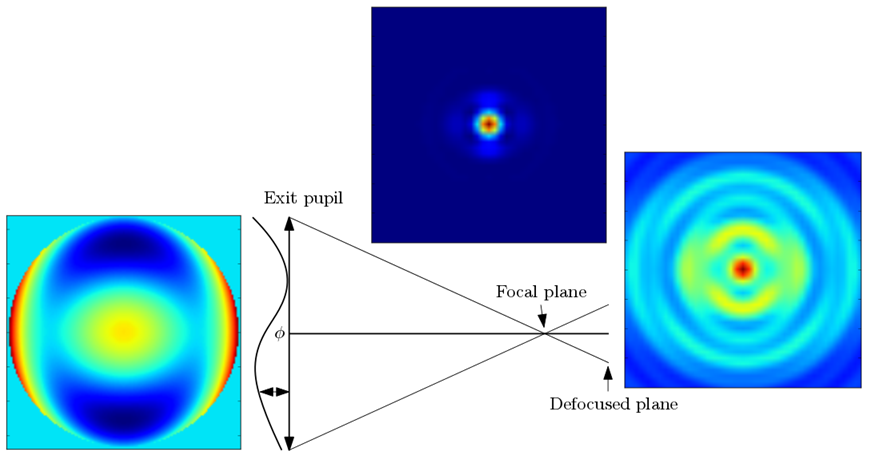
\includegraphics[width=0.8\textwidth,angle=0]{Figures/DiversityPrincipleM}
\decoRule
\caption{Schema of the phase diversity principle. The images from left to right are : the phase arriving on the exit pupil, the focused image and the defocused ($2\pi$) image.}
\label{fig:DiversityPrinciple}
\end{center}
\end{figure}

Unlike Shack-Hartmann wavefront reconstruction, which is a pupil plane technique, the phase diversity uses data acquired at the focal plane. Using the non-linear relation between the phase of the wavefront and the image, 

\begin{equation}
i(x,y) = (h_{optical}\otimes o)(x,y), \ with \ h_{optical}(x,y) = |\left[\mathcal{F}\left\lbrace A(\xi,\eta)e^{j\phi(\xi,\eta)} \right\rbrace\right](x,y)|^2,
\label{eqt:img-hopt}
\end{equation}

one can determine the phase, i.e. the aberrations present in the imaging system, by solving an inverse problem. The major difficulty of this technique is that, as one can see in eqt. \eqref{eqt:img-hopt}, there is not a unique solution to the problem at hand. This indetermination comes from the fact that the available detector can only sense the intensity of the wave, and not the wave itself, which is the modulus squared of the complex amplitude as exposed in section \ref{sec:ImSystem}. Thus, $\phi(\xi,\eta)$ and $\phi'(\xi,\eta)=-\phi(-\xi,-\eta)$ give the same PSF.
More specifically by decomposing the phase in its even and odd part and using the autocorrelation properties ($\Gamma_A = \Gamma_{A'}$ with $A'(t) = A*(-t)$), with only one image, one can not determine the sign of the phase even part. This leads to the introduction of a phase diversity to raise the indetermination. The idea is to add a known aberration $\delta\phi$ to the system and to use the two images to retrieve the phase of the wavefront.

The diversity between the two images is introduced for instance by defocusing one of the two images. In this work we will use this diversity, but having a more complex system, such has a deformable mirror, one could introduce any other even aberration such as an astigmatism, the only requirement is that the diversity introduced must have an even radial and azimuthal order. Figure \ref{fig:DiversityPrinciple} shows the principle of the phase diversity. Two images are acquired, one at the focal plane and another with a defocus. In this work, we introduce the defocus by sliding the detector along the z-axis, others use a beamsplitter and another detector \citep{mugnier_2006}.

The phase diversity is a technique that is sensible to chromatism, since it is based on diffraction. The non-linear relation that links the image and the phase depends also on the object. This renders the inverse problem to solve more complicated, but it allows to retrieve the phase, the object or both, when the object is unknown (most of the time). Furthermore, it is very simple optically, do not require a complex optical components to acquire the data, one just uses the detector in place. And it depends directly on the images so there is no noncommon-path aberration between the adaptive optic system and the scientific detector.

In this work, the final application of the phase diversity algorithm will be to correct for static aberration in an optical system. We will have knowledge of the object, since it will be a point source that we introduce with a laser or choose in the sky (a star).

\section[ONERA algorithm]{ONERA algorithm, \citet{mugnier_2006}}
\label{sec:ONERAalgo}

In this section, we will present briefly the phase diversity algorithm developed at ONERA since we test and use it to retrieve the phase and the aberrations in the experiment conducted in laboratory.

As explained in section \ref{sec:principle}, the phase diversity determines the phase of the wavefront, as well as the unknown object when needed, using two images of the same object with a phase diversity between each image. This gives the following equation system \citep[p.11]{mugnier_2006},

\begin{align}
\mathbf{i}_f &= \mathbf{h}_f \ast \mathbf{o} + \mathbf{n}_f \\
\mathbf{i}_d &= \mathbf{h}_d \ast \mathbf{o} + \mathbf{n}_d,
\label{eqt:systemEQT}
\end{align}

where the bold letters means that it is the sampled quantities, the indexes f and d means respectively focused and defocused and $\mathbf{n}$ regroups the photon and detector noise present on the image. Using the data available, this algorithm approaches the problem at hand with a statistic point of view. They estimate jointly the aberrations and the object \citep{Paxman1992}, which consist to compute the joint maximum \textit{a posteriori} (JMAP) estimator \citep[p.17]{mugnier_2006},

\begin{align}
(\hat{\mathbf{o}},\hat{\boldsymbol{\phi}})_{MAP} &= \underset{\mathbf{o},\boldsymbol{\phi}}{\mathrm{arg \ max}} \ p(\mathbf{i}_f,\mathbf{i}_d,\mathbf{o},\boldsymbol{\phi};\boldsymbol{\theta})\nonumber \\
&= \underset{\mathbf{o},\boldsymbol{\phi}}{\mathrm{arg \ max}} \ p(\mathbf{i}_f|\mathbf{o},\boldsymbol{\phi};\boldsymbol{\theta_n})p(\mathbf{i}_d|\mathbf{o},\boldsymbol{\phi};\boldsymbol{\theta_n})p(\mathbf{o};\boldsymbol{\theta_o})p(\boldsymbol{\phi};\boldsymbol{\theta_{\phi}}), 
\end{align}

where $p(\mathbf{i}_f,\mathbf{i}_d,\mathbf{o},\boldsymbol{\phi};\boldsymbol{\theta})$ is the joint probability density function of the two images $(\mathbf{i}_f,\mathbf{i}_d)$, the object $\mathbf{o}$ and the phase $\boldsymbol{\phi}$. It can also depend on a set of hyperparameters $\boldsymbol{\theta} = (\boldsymbol{\theta}_n,\boldsymbol{\theta}_o,\boldsymbol{\theta}_{\phi})$. $p(\mathbf{i}_k|\mathbf{o},\boldsymbol{\phi};\boldsymbol{\theta_n})$ is the likelihood of the image $\mathbf{i}_k$. $p(\mathbf{o};\boldsymbol{\theta_o})$ and $p(\boldsymbol{\phi};\boldsymbol{\theta_{\phi}})$ are the \textit{a priori} probability density functions of $\mathbf{o}$ and $\boldsymbol{\phi}$.

They assume that the noise is white and stationary with a variance $\sigma^2$ on each image. They take Gaussian prior probability distributions for the object and for the phase which they decompose on the Zernike polynomial basis, $\boldsymbol{\phi}(\mathbf{a})$, with $\mathbf{a}$ the vector containing the Zernike coefficients from $a_4$ to $a_{j_{max}}$, see \citet[p.18-19]{mugnier_2006} for the detailed expressions. Finally, the phase and the object are retrieved by maximizing the joint probability density function $p(\mathbf{i}_f,\mathbf{i}_d,\mathbf{o},\mathbf{a};\boldsymbol{\theta})$ or taking the logarithm of the latter they retrieve them by minimizing the following criterion,

\begin{align}
L&_{JMAP}(\mathbf{o},\mathbf{a},\boldsymbol{\theta}) \nonumber\\
&= -\mathrm{ln} \ p(\mathbf{i}_f,\mathbf{i}_d,\mathbf{o},\mathbf{a};\boldsymbol{\theta}) \nonumber \\
&= N^2\ \mathrm{ln}\ \sigma^2 + \frac{1}{2}\mathrm{ln}\ \mathrm{det}(R_0) + \frac{1}{2}\mathrm{ln}\ \mathrm{det}(R_a)\nonumber\\
& \ + \frac{1}{2\sigma^2}(\mathbf{i}_f -H_f\mathbf{o})^t(\mathbf{i}_f -H_f\mathbf{o})+ \frac{1}{2\sigma^2}(\mathbf{i}_d - H_d \mathbf{o})^t(\mathbf{i}_d-H_d\mathbf{o})\nonumber\\
& \ + \frac{1}{2}(\mathbf{o}-\mathbf{o}_m)^t R_o^{-1}(\mathbf{o}-\mathbf{o}_m) + \frac{1}{2}\mathbf{a}^tR_a^{-1}\mathbf{a} + A,
\end{align}

where $N^2$ is the number of pixels in the image, $\mathbf{o}_m$ and $R_o$ are the mean object and its covariance matrix, $R_a$ is the covariance matrix of the aberrations, $H_k$ is the matrix representing the discrete convolution by the sampled $\mathbf{h}$ and A is a constant.

In order to simplify and fasten the computation, they rewrite the criterion replacing $\mathbf{o}$ by its estimator $\hat{\mathbf{o}}(\mathbf{a},\boldsymbol{\theta})$ obtained by cancelling the derivative of $L_{JMAP}$ with respect to $\mathbf{o}$, and they move to the Fourier domain, see eqt. (24) of \citet[p.21]{mugnier_2006}.


\section{Analytical algorithm}
\label{sec:AnAlgo}

This algorithm uses an analytical method to retrieve the phase of the wavefront \textbf{induced by a known point source object}. We assume the object known, because we want to correct for the static aberrations present in the optical system to the scientific detector and thus we use a point source to illuminate the optical system, either a star or a laser.

As we have seen in section \ref{sec:ImSystem}, the PSF of an optical system correspond to the image it gives of a point source,

\begin{equation}
PSF(x,y) = \frac{1}{S_p^2}|\left[\mathcal{F}\left\lbrace P(\xi,\eta)A(\xi,\eta)e^{-j\phi(\xi,\eta)} \right\rbrace\right](x,y)|^2,
\label{eqt:PSF}
\end{equation}

where $P(\xi,\eta)$ is the exit pupil function, $A(\xi,\eta)$ is the amplitude of the wave through the exit pupil, $\phi(\xi,\eta)$ is the phase of the wavefront and $S_p$ is the exit pupil surface. In the following we will omit the coordinates to simplify the notation. The unit of the PSF is directly the Strehl ratio. Under the assumption that we have weak aberrations, we can expand the exponential term,

\begin{equation}
exp(-j\phi)\approx 1 - j\phi - \frac{\phi^2}{2} + O(\phi^3),
\label{eqt:expansionPhase}
\end{equation}

replacing the exponential by its expansion in eqt.\eqref{eqt:PSF} leads to,

\begin{equation}
S_p^2 PSF \cong |\mathcal{F}\left\lbrace PA (1-j\phi-\frac{\phi^2}{2}) \right\rbrace|^2
\label{eqt:PSFwthPhaseExpand}
\end{equation}

Developing eqt. \eqref{eqt:PSFwthPhaseExpand}, keeping only the terms up to the second order, assuming that the amplitude through the pupil $A(\xi,\eta)$ is constant and unitary since we have a point source object and using the well known complex relations,

\begin{align}
a + a^* &= 2 \Re \lbrace a \rbrace \nonumber \\
a - a^* &= 2j \Im \lbrace a \rbrace, \nonumber
\end{align}

we obtain the following relation,

\begin{equation}
S_p^2 PSF \cong |\widetilde{P}|^2 + |\widetilde{P\phi}|^2 + 2\Im\lbrace \widetilde{P^*}\widetilde{P \phi}\rbrace - 2\Re\lbrace \widetilde{P^*}\widetilde{P \phi^2}\rbrace
\label{eqt:devPSFwthPhaseExpand}
\end{equation}

Defining $\Delta PSF$ as the difference between eqt. \eqref{eqt:devPSFwthPhaseExpand} for an arbitrary optical system and its perfect equivalent, we obtain the following expression,

\begin{equation}
\Delta PSF = S_p^2 PSF - S_p^2 PSF_{perfect} = |\widetilde{P\phi}|^2 + 2\Im\lbrace \widetilde{P^*}\widetilde{P \phi}\rbrace - 2\Re\lbrace \widetilde{P^*}\widetilde{P \phi^2}\rbrace,
\label{eqt:DeltaPSF}
\end{equation}

where $S_p^2 PSF_{perfect}$ is equal for a equivalent perfect system with the same pupil to $|\widetilde{P}|^2$. One can decompose $\phi$ into its even and odd phase, $\psi$ and $\gamma$ respectively,

\begin{equation}
\phi = \psi + \gamma
\label{eqt:Phidecomposed}
\end{equation}

Developing eqt. \eqref{eqt:DeltaPSF} after replacing $\phi$ by its decomposition and using the properties of the Fourier transform of real and purely even or odd functions, we get the following expression,

\begin{equation}
\Delta PSF = |\widetilde{P\psi}|^2 + |\widetilde{P\gamma}|^2 + 2\Im\lbrace \widetilde{P^*}\widetilde{P \gamma}\rbrace - \Re\lbrace \widetilde{P^*}\widetilde{P \psi^2}\rbrace- \Re\lbrace \widetilde{P^*}\widetilde{P \gamma^2}\rbrace
\label{eqt:DeltaPSFdeveloped}
\end{equation}

We can decompose $\Delta PSF$ into its even and odd components,

\begin{align}
\Delta PSF_{even} &= |\widetilde{P\psi}|^2 + |\widetilde{P\gamma}|^2 - \Re\lbrace \widetilde{P^*}\widetilde{P \psi^2}\rbrace- \Re\lbrace \widetilde{P^*}\widetilde{P \gamma^2}\rbrace, \label{eqt:DeltaPSFeven}\\
\Delta PSF_{odd} &= 2\Im\lbrace \widetilde{P^*}\widetilde{P \gamma}\rbrace \label{eqt:DEltaPSFodd},
\end{align}

This equation system shows that we can retrieve the odd part of the phase easily with eqt. \eqref{eqt:DEltaPSFodd}. But eqt. \eqref{eqt:DeltaPSFeven} clearly reveals the indetermination of the phase retrieval with only one image, as the sign of the even part of $\phi$ can not be determine. In order to raise this indetermination, as exposed in section \ref{sec:principle}, we need to introduce a phase diversity $\delta\phi$. We can modify the pupil function $P$ in order to take into account this introduced diversity,

\begin{equation}
P_{\delta} \equiv P e^{-j\delta\phi} = P(cos(\delta\phi)-jsin(\delta\phi)) = P(C-iS) 
\label{eqt:pupilDeltaphi}
\end{equation}

The expression of $\Delta PSF_{\delta\phi}$, which is the $\Delta PSF$ at the defocus plane, is found by replacing $P$ by $P_{\delta}$ in eqt. \eqref{eqt:DeltaPSFdeveloped}, we give directly the expressions of the even and odd components by taking into account that the phase is only define on the pupil ($P\phi=\phi$) to simplify the reading,

\begin{align}
\Delta PSF_{\delta\phi, even} &= |\widetilde{C\psi}|^2 + |\widetilde{C\gamma}|^2 +|\widetilde{S\psi}|^2 + |\widetilde{S\gamma}|^2 -2\widetilde{PC}^*\widetilde{S\psi}+2\widetilde{PS}^*\widetilde{C\psi} \nonumber\\
&-\widetilde{PC}^*\widetilde{C\psi^2}-\widetilde{PC}^*\widetilde{C\gamma^2}-\widetilde{PS}^*\widetilde{S\psi^2}-\widetilde{PS}^*\widetilde{S\gamma^2} \label{eqt:deltaPSFevenDef}\\
\Delta PSF_{\delta\phi, odd} &= 2\widetilde{C\psi}^*\Im\lbrace\widetilde{S\gamma}\rbrace+2\Im\lbrace\widetilde{C\gamma}^*\rbrace\widetilde{S\psi}+2\widetilde{PC}^*\Im\lbrace\widetilde{C\gamma}\rbrace+2\widetilde{PS}^*\Im\lbrace\widetilde{S\gamma}\rbrace \nonumber\\
&+2j\widetilde{PC}^*\widetilde{S\psi\gamma}-2j\widetilde{PS}^*\widetilde{C\psi\gamma}.\label{eqt:deltaPSFoddDef}
\end{align}

Eqt. \eqref{eqt:DEltaPSFodd}, eqt. \eqref{eqt:deltaPSFevenDef} and eqt. \eqref{eqt:deltaPSFoddDef} allow to retrieve the complete phase of the optical system under the assumption of weak aberrations.

\chapter{Phase Diversity Experiment} 
\label{ch:PDExp}

Here, we will describe the experiment put in place in the optical laboratory at the HEIG-VD to reconstruct wavefronts with unknown static aberrations introduced using phase screens. At first, we study the  behaviour of the phase diversity algorithm put in place by \citet{mugnier_2006} at ONERA with respect to number of averaging images, in other words noise level, and number of Zernike coefficients retrieved. Then we test the algorithm using a known aberration introduced by a parallel plane plate in the beam comparing the result to Zemax simulation. And finally, we introduce the phase screen to have random aberrations in the pupil and try to compare the phase diversity results with the Shack Hartman wavefront sensor results.

\section{Experimental Setup}
\label{sec:ExpSetup}
\begin{figure}
\begin{center}
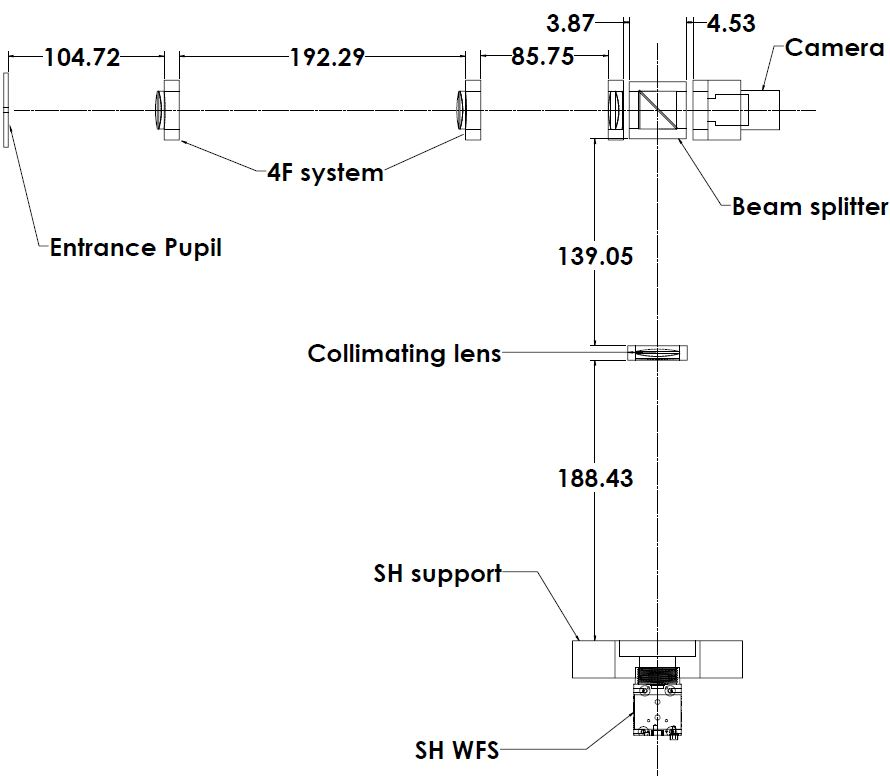
\includegraphics[width=0.8\textwidth,angle=0]{Figures/setupSchema.JPG}
\decoRule
\caption[Experimental Setup Schema]{Experimental setup schema with the relevant distances, \citep{Bouxin_PDM}.}
\label{fig:setupSchema}
\end{center}
\end{figure}

The design of the experiment was already done by \citet{Bouxin_PDM}. The system is built according to her plans and specifications. Figure \ref{fig:setupSchema} shows the schema of the experimental setup.

The experiment is mounted on a pressurized legs optical table. The assembly contains six main components : a light source, an entrance pupil, an imaging system, a converging lens to focus the beam on the camera, a camera and a wavefront sensor.

\subsection{Light source}
\label{subsec:LigthSource}

\begin{minipage}{\linewidth}
\begin{wrapfigure}{r}{0.4\textwidth}
\centering
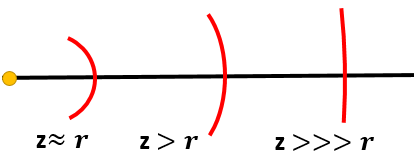
\includegraphics[width=0.4\textwidth]{Figures/WFdistantSource.PNG}
\decoRulewrapFig
\caption[Wavefront curvature]{Wavefront curvature for different point source's distances, \textit{z}. \textit{r} represents the characteristic size of the arc of interest.}
\label{fig:WFdistantSource}
\end{wrapfigure}

The final application of the phase diversity will be to characterize the optical aberrations induced by the imperfect optical path to a scientific detector of a telescope. For this reason, the light source has to simulate a distant star aberration-free wavefront. A distant star wavefront is considered planar since the object distance, z, is far greater than the telescope size, r, see Fig. \ref{fig:WFdistantSource}. The source of our experiment must then be characterized by a planar wavefront.

In order to obtain such a planar wavefront at the entrance pupil, the light source consist of a "pigtailed laser diode", a f=11mm converging lens, a pinhole and a f=200 mm converging lens, see Table \ref{tab:optComp}. The pigtailed laser diode emits a Gaussian beam centred at 637.5 nm slightly diverging. The converging lens concentrates the beam at the center of the 10$\mu$m pinhole to filter the noise. The second converging lens collimates the beam, obtaining a collimated beam with a planar wavefront, see Fig. \ref{fig:sourceRayTracing} and \ref{fig:pinholeEffect}.

\end{minipage}

\begin{figure}
\centering
    \begin{subfigure}{0.5\textwidth}
        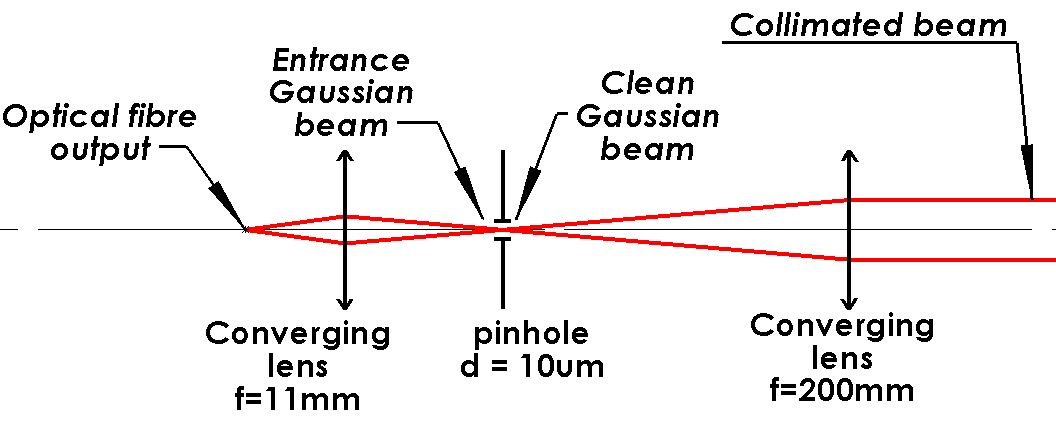
\includegraphics[width=\textwidth]{Figures/source.png}
        \caption{Source ray tracing.}
        \label{fig:sourceRayTracing}
    \end{subfigure}
    \quad
    \begin{subfigure}{0.3\textwidth}
        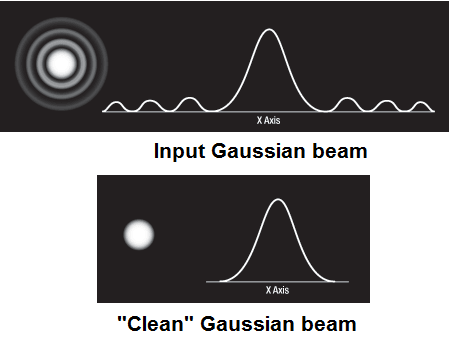
\includegraphics[width=\textwidth]{Figures/pinholeEffect.png}
        \caption{Beam view before and after the pinhole, \citep{SpatialFilters}.}
        \label{fig:pinholeEffect}
    \end{subfigure}
    \decoRule
    \caption{Source schema and pinhole effect on the beam.}
\end{figure}

\subsection{Entrance pupil}
\label{subsec:EntrancePupil}

The entrance pupil of our optical system is a circular aperture of 3.2 mm diameter placed after the collimating lens of the light source. It is milled in a metal plate and centred in his support, to avoid positioning with a XY table. The diameter is chosen in available material to fit in the different detector's surfaces.

\subsection{Pupil imaging system}
\label{subsec:pupilImSystem}

The phase diversity technique requires PSFs images as input, which means that the beam as to be focused onto the detector surface. To analyse the aberration in the pupil plane, one needs to focus an image of the beam passing through the entrance pupil. The simplest assembly to achieve this goal is the 4F system, which consist of two converging lenses of focal 100 mm. The two lenses are separated by 200 mm, see Fig. \ref{fig:setupSchema}. This places the image of the entrance pupil 100 mm after the second converging lens.

\subsection{Detectors}
\label{subsec:Detectors}

The image of the entrance pupil, obtained with the 4F system, is focused onto a CMOS Ximea camera by a f = 80 mm converging lens to acquire the PSFs for the phase diversity wavefront retrieval. The camera has a surface composed by 1280x1024 pixels of 5.3 $\mu$m, see Appendix \ref{app:ximeaCam}. It is mounted on sliding support in order to be able to acquire in/out-of-focus images. A beam splitter is placed in the converging beam to separate it in two. The second beam is collimated and a Shack-Hartman WFS is placed on the entrance pupil image plane, to check the results of the phase diversity wavefront retrieval. The Shack-Hartman WFS has a 39 X 31 lenslets grid and a CCD with a resolution of 1280x1024 pixels of 4.65 $\mu$m, see Appendix \ref{app:SHwfs}. 

\begin{table}
\caption{Optical Components}
\label{tab:optComp}
\centering
\begin{tabular}{|l|l|l|c|}
\hline
\textbf{\#}& \textbf{Components} & \textbf{Model} & \textbf{Reference} \\\hline
1 & Pigtailed laser diode & Thorlabs, LPS-635-FC & \ref{app:pigtailedLaserDiode} \\\hline
2 & Converging lens, f = 11 mm & Thorlabs, A220TM-A & \ref{app:CL11} \\\hline
3 & Pinhole, 10 $\mu$m & Thorlabs, P10S & \ref{app:pinhole10microns} \\\hline
4 & Converging lens, f = 200 mm & Thorlabs, AL100200 & \ref{app:CL200} \\\hline
5 & 3.2 mm Hole milled in metal sheet & ... & ... \\\hline
6 & Converging lens, f = 100 mm & Thorlabs, AC254-100-A & \ref{app:CL100} \\\hline
7 & Converging lens, f = 80 mm & & \\\hline
8 & Camera CMOS & Ximea, MQ013MG-E2 & \ref{app:ximeaCam} \\\hline
9 & Converging lens, f = 100 mm & & \\\hline
10 & Shack-Hartman WFS & Thorlabs, WFS150-5C & \ref{app:SHwfs} \\\hline
\end{tabular}
\end{table}

\section{Data Acquisition}
\label{sec:DataAcquis}

\subsection{Ximea Camera}
\label{subsec:acquisXimCam}

The ONERA algorithm takes at least one focused and one defocused PSFs, as described in section \ref{subsec:OneraAlgoImp}. The PSFs are acquired using a python script which uses an open-source library to control the ximea camera, \verb|pyXimea|\footnote{\url{https://github.com/pupil-labs/pyximea}}, available on GitHub. The acquisition is done following these steps : 

\begin{enumerate}

\item The first step in order to acquire PSFs is to determine the position of the camera's focus point using the python script \verb|AlignementScriptXimeaCamera.py|, see Appendix \ref{subapp:AlignementScriptXimeaCamera}. This script let's you acquire consecutively PSFs at different camera's positions and computes their FWHM. It finally returns the minimum FWHM and the camera's position, see Figure \ref{subfig:28092017AlignementXimeaPSFs} and \ref{subfig:28092017AlignementXimeaPos}.

\begin{figure}
\centering
    \begin{subfigure}{\textwidth}
        \includegraphics[width=\textwidth]{../../../fig/alignement/28092017AlignementXimeaPSFs.png}
        \caption{PSFs taken during the alignment procedure, each image is taken at an other camera position.}
        \label{subfig:28092017AlignementXimeaPSFs}
    \end{subfigure}
    \\
    \begin{subfigure}{0.6\textwidth}
        \includegraphics[width=\textwidth]{../../../fig/alignement/28092017AlignementXimeaPos.png}
        \caption{FWHM of the PSFs as a function of the camera's position. The minimum is at $11.55$ mm}
        \label{subfig:28092017AlignementXimeaPos}
    \end{subfigure}
    \decoRule
    \caption{Example of the results of an alignment procedure}
\end{figure}

\item Once the focus point position of the camera is determined, the acquisition of the data is possible. The acquisition script is called \verb!AcquisAndSaveXimea.py!, see Appendix \ref{subapp:AcquisAndSaveXimea}.

\item The user needs to set the main parameters before acquiring. They are the number of images on which to average, the size of the final PSFs, the position of the focus point on the sliding system and the initial guess to fit the 2D Gaussian on the PSF to find its center. The initial guess can be made using the Ximea camera software, called \verb!xiCamTool!, with which one gets a live feedback of the camera.

\item Then the running program ask the user what he needs to do after having made a sound. The first thing the user needs to do is to place the camera at the focus point and turn on the LED in order to set the optimal exposure time in order to avoid saturation.

\item Finally the acquiring sequence begins, the program ask the user to shut down and turn on the source as the user acquire the different images to get the dark images and the PSF images. The user needs to manually displace the camera to get the defocused PSFs. The program computes the positions to get a $2\pi$ P2V defocus dephasing.

\end{enumerate}

Many functions, used in the two scripts described above, are coded in the script \verb!functionsXimea.py!, see Appendix \ref{subapp:functionsXimea}.

\subsection{Shack-Hartmann WFS}
\label{subsec:acquisSHwfs}

The Shack-Hartmann wavefront sensor acquisition is done with the company software. The acquired data are the Zernike coefficients and the reconstructed wavefront computed following the principle described in section \ref{subsec:SHprinciple}. Their is a few parameters that the user can set : the exposure time (there is also an auto set), the number of averaging images (1 up to 300) and the focus points reference of the micro-lenses array. 

The data are saved manually in a \textit{.csv} file. I coded an IDL script to read and average the Shack-Hartmann data, in order to be able to analyse them and compare the result with the phase diversity, see Appendix \ref{subapp:readAndAverageSHdata} and \ref{subapp:readSHWFSdata}. 

\section{Results}
\label{sec:Results}

This section presents the results of the phase diversity experiment, with the introduction of different sources of aberration. We will first present the results of the ONERA algorithm test, then we will compare the phase diversity retrieval with a calibrated aberration and finally we will introduce random static aberration with the phase screen and compare the results to the Shack-Hartmann wavefront sensor results.

\subsection{ONERA Phase Diversity test}
\label{subsec:ONERAPDtest}

The motivation of this test was to better understand the behaviour of the ONERA phase diversity algorithm with respect to the different parameters that could influence its results, such as the noise present in the PSFs, the number of Zernike coefficients returned for the modal mode and the error on the defocused distance of the PSFs.

\begin{figure}
\begin{center}
\includegraphics[width=0.6\textwidth,angle=0]{../../../fig/PD/noise_study/NoiseCurveXimea}
\decoRule
\caption{Noise level as a function of the number of averaging images acquired with $\sim$ 300 $\mu$s exposition time. The noise level is computed as the mean of the standard deviation of every pixel divided by the maximum of the focused PSF.}
\label{fig:NoiseCurve}
\end{center}
\end{figure}

To study the noise, we acquire PSFs with 25 different numbers of averaging images going from 10 to 5000. The noise level is computed as the ratio between the mean pixel standard deviation and the PSF maximum. The Ximea detector has a noise curve visible in Figure \ref{fig:NoiseCurve}. The noise curve is computed with the noise level of the focused PSFs. It follows an exponential law with the number of averaging images. The noise level varies from $\sim 1\mathrm{e}-3$ to $\sim 8\mathrm{e}-5$, for 10 and 5000 images respectively. Having the noise curve of the detector, we can study empirically how it influences the phase diversity results. 

\begin{figure}
\centering
    \begin{subfigure}{0.8\textwidth}
        \includegraphics[width=\textwidth]{../../../fig/PD/noise_study/ZernikeCoef_J_differentNbrAveraging.png}
        \caption{Zernike coefficients $a_j$ as a function of $j$ the Zernike index of the 25 modal and zonal phase retrievals, in blue and red respectively.}
        \label{subfig:ZernikeCoef_J_differentNbrAveragingjmax30}
    \end{subfigure}
    \\
    \begin{subfigure}{0.5\textwidth}
        \includegraphics[width=\textwidth]{../../../fig/PD/noise_study/Boxplot_Aj_j_jmax30.png}
        \caption{Boxplot of the 25 Zernike coefficients $a_j$ of the different phase retrievals computed with the different averaging numbers of images as a function of the Zernike index $j$.}
        \label{subfig:Boxplot_Aj_j_jmax30}
    \end{subfigure}
    \decoRule
    \caption{Results of the phase retrievals computed with the 25 different noise levels. The phase retrievals are done with a $j_{max} = 30$}
\end{figure}

Figures \ref{subfig:ZernikeCoef_J_differentNbrAveragingjmax30} and \ref{subfig:Boxplot_Aj_j_jmax30} presents the results of the 25 different retrievals. As one can see there is some spread due to the different noise levels present in the PSFs given to the algorithm. The biggest standard deviation on a Zernike coefficient is smaller than 6 nm. And there can be up to 20 nm of maximal difference between the $a_j$'s as one can see on Figure \ref{subfig:Boxplot_Aj_j_jmax30}. The spherical aberration, $a_{11}$, has the biggest standard deviation and range of values. This shows that the PSFs noise levels have an impact on the retrieval and that not all Zernike coefficient are affected in the same way. One reassuring point is the good correspondence between the modal and zonal retrievals.

\begin{figure}
\begin{center}
\includegraphics[width=\textwidth,angle=0]{../../../fig/PD/noise_study/WavefrontsNoiseStudy}
\decoRule
\caption{Reconstructed wavefronts for two different number of averaging images, 10 and 3500, left and right column respectively. The two first line are modal retrieval with $j_{max}=30$ and $j_{max}=200$ and the last line is the zonal retrieval.}
\label{fig:WavefrontsNoiseStudy}
\end{center}
\end{figure}

Furthermore, looking at the reconstructed wavefronts in Figure \ref{fig:WavefrontsNoiseStudy}, one can see the effect of noise in the PSFs and how important is the choice of $j_{max}$ for the modal reconstruction. Indeed, for the wavefronts reconstructed using $j_{max}=30$, the retrieved structures are similar, however for $j_max=200$ there are more structures in the retrieval done on the PSFs with 10 averaging images. This shows that the noise has a signal at high spatial frequencies. The zonal retrieval shows it clearly, the reconstruction is significantly different between 10 and 3500 averaging images. The averaging over a large number of acquisition smooth out the noise structures that perturbs the reconstruction. Also as said above with the Zernike coefficients is still valid for the wavefront, the two retrieval method gives similar results. But Figure \ref{fig:WavefrontsNoiseStudy} shows that the choice of $j_{max}$ is important if one wants to use the reconstructed wavefronts.

\newpage
\subsection{Parallel plane plate}
\label{subsec:ParPlanePlate}

The first source of aberration studied in this work is a tilted parallel plane plate which is used as a calibrated source of astigmatism.
 

%----------------------------------------------------------------------------------------
%	THESIS CONTENT - APPENDICES
%----------------------------------------------------------------------------------------

\appendix % Cue to tell LaTeX that the following "chapters" are Appendices

% Include the appendices of the thesis as separate files from the Appendices folder
% Uncomment the lines as you write the Appendices

% Appendix A

\chapter{Optical Component Datasheets}
\label{AppendixA} 

\section{Pigtailed laser diode}
\label{app:pigtailedLaserDiode}
\includegraphics[width=\textwidth]{../../componentDatasheet/LPS-635-FC-SpecSheet.pdf}
Source : \url{www.thorlabs.com}

\section{Converging lens A220TM-A, f = 11 mm}
\label{app:CL11}
\includegraphics[width=\textwidth]{../../componentDatasheet/A220TM-AutoCADPDF.pdf}
Source : \url{www.thorlabs.com}

\section{Pinhole 10 $\mu$m}
\label{app:pinhole10microns}
\includegraphics[width=\textwidth]{../../componentDatasheet/P10S-AutoCADPDF.pdf}
Source : \url{www.thorlabs.com}

\section{Converging lens AL100200, f = 200 mm}
\label{app:CL200}
\includegraphics[width=\textwidth]{../../componentDatasheet/AL100200-AutoCADPDF.pdf}
Source : \url{www.thorlabs.com}

\section{Converging lens AC254-100-A, f = 100 mm}
\label{app:CL100}
\includegraphics[width=\textwidth]{../../componentDatasheet/AC254-100-A-AutoCADPDF.pdf}
Source : \url{www.thorlabs.com}

\section{Ximea Camera, MQ013MG-E2}
\label{app:ximeaCam}
\begin{center}
\includegraphics[width=0.5\textwidth]{../../componentDatasheet/ximeaPic.png}
\includegraphics[width=0.5\textwidth]{../../componentDatasheet/ximeaSpec.png}
\end{center}
Source : \url{www.ximea.com/en/products/usb3-vision-cameras-xiq-line/mq013mg-e2}

\section{Shack-Hartmann wavefront sensor, WFS150-5C}
\label{app:SHwfs}
\includegraphics[width=\textwidth]{../../componentDatasheet/WFS150-5C.png}
Source : WFS Series Operation Manual, \url{www.thorlabs.com}


\chapter{Python Code}
\label{AppPythonCode}

\section{Phase Diversity analytical algorithm code}
\label{app:phaseDiversityanAlgoCode}

\subsection{phaseDiversity3PSFs.py}
\label{subapp:phaseDiversity3PSFs}

\begin{lstlisting}
#Class phaseDiversity object to retrieve the phase in the pupil from two psfs in/out of focus

import numpy as np
import fs
import myExceptions
import PSF as psf

class phaseDiversity3PSFs(object):

    def __init__(self,inFoc,outFocpos,outFocneg,deltaZ,lbda,pxsize,F,pupilRadius,jmin,jmax):
#        
#        input:
#        inFoc,outFocpos,outFocneg are the 3 squared PSFs data, (focused, defocused positiv and defocused negative)
#        deltaZ is the displacement of the detector to acquire the two defocused PSFs
#        lbda is the wavelength of the incoming light
#        pxsize is the pixel size of the detector
#        F is the focal length of the imaging system
#        pupilRadius is the radius of the exit pupil
#        jmin and jmax gives the boundary on the js to retrieve
        
        print 'phaseDiversity ...'        
        
        #PSF
        self.inFoc = inFoc
        self.outFocpos = outFocpos
        self.outFocneg = outFocneg
        shapeinFoc = np.shape(self.inFoc)
        shapeoutFocpos = np.shape(self.outFocpos)
        shapeoutFocneg = np.shape(self.outFocneg)
        if shapeinFoc == shapeoutFocpos and shapeinFoc == shapeoutFocneg:
            self.shape = shapeinFoc
        else:
            raise myExceptions.PSFssizeError('the shape of the in/out PSFs is not the same',[shapeinFoc,shapeoutFocpos])
        if shapeinFoc[0]==shapeinFoc[1] and np.mod(shapeinFoc[0],2)==0:
            self.N = shapeinFoc[0]
        else:
            raise myExceptions.PSFssizeError('Either PSF is not square or mod(N,2) != 0',shapeinFoc)
            
        # properties   
        self.deltaZ = deltaZ
        self.lbda = lbda
        self.pxsize = pxsize
        self.F = F
        self.pupilRadius = pupilRadius
        self.dxp = self.F*self.lbda/(self.N*self.pxsize)
        self.rad = int(np.ceil(self.pupilRadius/self.dxp))
        if 2*self.rad > self.N/2.:
            raise myExceptions.PupilSizeError('Npupil (2*rad) is bigger than N/2 which is not correct for the fft computation',[])
        self.NyquistCriterion()
        self.jmin = jmin
        self.jmax = jmax
        self.oddjs = fs.getOddJs(self.jmin,self.jmax)
        self.evenjs = fs.getEvenJs(self.jmin,self.jmax)
        
        # result computation
        self.result = self.retrievePhase()

    def NyquistCriterion(self):
        deltaXfnyq = 0.5*self.lbda/(2*self.pupilRadius)
        deltaXf = self.pxsize/self.F
        if deltaXfnyq < deltaXf : raise myExceptions.NyquistError('the system properties do not respect the nyquist criterion',[])

    def retrievePhase(self):
        y1,A1 = self.initiateMatrix1()
        results1 = np.linalg.lstsq(A1,y1)
        ajsodd = results1[0]
        A1tA1inv= np.linalg.inv(np.matmul(np.transpose(A1),A1))
        n_p = y1.size-1
        ste1 = np.sqrt(results1[1]/n_p * np.diagonal(A1tA1inv))
        
        deltaphi = fs.deltaPhi(self.N,self.deltaZ,self.F,2*self.pupilRadius,self.lbda,self.dxp)
        y2,A2 = self.initiateMatrix2(deltaphi)
        results2 = np.linalg.lstsq(A2,y2)
        ajseven = results2[0]
        A2tA2inv= np.linalg.inv(np.matmul(np.transpose(A2),A2))
        n_p = y2.size-1
        ste2 = np.sqrt(results2[1]/n_p * np.diagonal(A2tA2inv))

        js = np.append(self.oddjs,self.evenjs)
        ajs = np.append(ajsodd,ajseven)
        ajsSte = np.append(ste1,ste2)

        Ixjs = np.argsort(js)
        result = {'js': js[Ixjs], 'ajs': ajs[Ixjs], 'ajsSte': ajsSte[Ixjs]} #,'wavefront':phase}
        return result

    def initiateMatrix1(self):
        deltaPSFinFoc = self.CMPTEdeltaPSF()
        y1 = fs.y1(deltaPSFinFoc)
        A1 = np.zeros((self.N**2,len(self.oddjs)))
        for ij in np.arange(len(self.oddjs)):
            phiJ = fs.f1j(self.oddjs[ij],self.N,self.dxp,self.pupilRadius)
            A1[:,ij] = phiJ
        return y1,A1
    
    def initiateMatrix2(self,deltaphi):
        deltaPSFoutFocpos,deltaPSFoutFocneg = self.CMPTEdeltaPSF(self.deltaZ)
        y2 = fs.y2even(fs.getEvenPart(deltaPSFoutFocpos),fs.getEvenPart(deltaPSFoutFocneg))
        A2 = np.zeros((self.N**2,len(self.evenjs)))
        for ij in np.arange(len(self.evenjs)):
            phiJ = fs.f2jeven(self.evenjs[ij],self.N,deltaphi,self.dxp,self.pupilRadius)
            A2[:,ij] = phiJ
        return y2,A2

    def CMPTEdeltaPSF(self,deltaZ=[]):
        if not deltaZ:
            PSF = psf.PSF([1],[0],self.N,self.dxp,self.pupilRadius)
            return PSF.Sp**2*self.inFoc - PSF.Sp**2*PSF.PSF
        else:
            P2Vdephasing = np.pi*self.deltaZ/self.lbda*(2*self.pupilRadius/self.F)**2/4.
            a4 = P2Vdephasing/2./np.sqrt(3)
            PSF = psf.PSF([4],[a4],self.N,self.dxp,self.pupilRadius)
            return [PSF.Sp**2*self.outFocpos - PSF.Sp**2*PSF.PSF,PSF.Sp**2*self.outFocneg - PSF.Sp**2*PSF.PSF]
\end{lstlisting}

\subsection{fs.py}
\label{subapp:fs}
\begin{lstlisting}
#functions to compute the matrix element of the system of equations Ax = b
import zernike as Z
import phasor as ph
import numpy as np

def f1j(j,N,dxp,pupilRadius): # 1: phij's of matrix A to find a_j odd
    Zj = Z.calc_zern_j(j,N,dxp,pupilRadius)
    FFTZj = scaledfft2(Zj,dxp)

    Lp = N*dxp
    xp = np.arange(-Lp/2,Lp/2,dxp)
    yp = xp

    [Xp,Yp]=np.meshgrid(xp,yp)
    
    pupil = np.float64(np.sqrt(Xp**2+Yp**2)<=pupilRadius)
    FFTPupil = scaledfft2(pupil,dxp)

    return np.ravel(2 * np.real(FFTPupil) * np.imag(FFTZj))

def f2j(j,N,jsodd,ajsodd,deltaphi,dxp,pupilRadius): # 2: phij's of matrix A to find a_j even
    #Get the jth zernike polynomials values on a circular pupil of radius rad
    Zj = Z.calc_zern_j(j,N,dxp,pupilRadius)

    #compute the different 2Dfft given in the equations of deltaPSF
    cosZj = np.cos(deltaphi)*Zj
    sinZj = np.sin(deltaphi)*Zj
    FFTcosZj =  scaledfft2(cosZj,dxp)
    FFTsinZj =  scaledfft2(sinZj,dxp)

    #odd phase
    oddPhasor = ph.phasor(jsodd,ajsodd,N,dxp,pupilRadius)
    oddPhase = oddPhasor.phase
    pupil = oddPhasor.pupil
    cosOddPhase = pupil*np.cos(deltaphi)*oddPhase
    sinOddPhase = pupil*np.sin(deltaphi)*oddPhase
    FFTcosOddPhase =  scaledfft2(cosOddPhase,dxp)
    FFTsinOddPhase =  scaledfft2(sinOddPhase,dxp)

    #2Dfft of pupil function times sin(deltaPhi) and cos(deltaPhi)
    pupilSin = pupil*np.sin(deltaphi)
    pupilCos = pupil*np.cos(deltaphi)
    FFTPupilSin =  scaledfft2(pupilSin,dxp)
    FFTPupilCos =  scaledfft2(pupilCos,dxp)

    FFTsinZjOddPhase = scaledfft2(sinZj*oddPhase,dxp)
    FFTcosZjOddPhase = scaledfft2(cosZj*oddPhase,dxp)

    return np.ravel(2*np.imag(np.conj(FFTcosZj) * FFTsinOddPhase + FFTsinZj * np.conj(FFTcosOddPhase)
            - np.conj(FFTPupilCos) * FFTsinZjOddPhase + np.conj(FFTPupilSin) * FFTcosZjOddPhase))
            
def f2jeven(j,N,deltaphi,dxp,pupilRadius): # 2: phij's of matrix A to find a_j even
    #Get the jth zernike polynomials values on a circular pupil of radius rad
    Zj = Z.calc_zern_j(j,N,dxp,pupilRadius)
    Phasor = ph.phasor([1],[0],N,dxp,pupilRadius)
    pupil = Phasor.pupil
    #compute the different 2Dfft given in the equations of deltaPSF
    cosZj = pupil*np.cos(deltaphi)*Zj
    sinZj = pupil*np.sin(deltaphi)*Zj
    FFTcosZj =  scaledfft2(cosZj,dxp)
    FFTsinZj =  scaledfft2(sinZj,dxp)
    #2Dfft of pupil function times sin(deltaPhi) and cos(deltaPhi)
    pupilSin = pupil*np.sin(deltaphi)
    pupilCos = pupil*np.cos(deltaphi)
    FFTPupilSin =  scaledfft2(pupilSin,dxp)
    FFTPupilCos =  scaledfft2(pupilCos,dxp)

    return np.ravel(-4*np.real(np.conj(FFTPupilCos)*FFTsinZj-np.conj(FFTPupilSin)*FFTcosZj))

def y1(deltaPSFinFoc): #1: yi's of y to find a_j odd
    #compute the odd part of delta PSF
    oddDeltaPSF = getOddPart(deltaPSFinFoc)
    return np.ravel(oddDeltaPSF)

def y2(deltaPSFoutFoc,N,jsodd,ajsodd,deltaphi,dxp,pupilRadius): # 2: yi's of y to find a_j even
    oddDeltaPSF = getOddPart(deltaPSFoutFoc)
    oddPhasor = ph.phasor(jsodd,ajsodd,N,dxp,pupilRadius)
    oddPhase = oddPhasor.phase

    pupilSin = oddPhasor.pupil*np.sin(deltaphi)
    pupilCos = oddPhasor.pupil*np.cos(deltaphi)
    FFTPupilSin =  scaledfft2(pupilSin,dxp)
    FFTPupilCos =  scaledfft2(pupilCos,dxp)
    cosOddPhase = oddPhasor.pupil*np.cos(deltaphi)*oddPhase
    sinOddPhase = oddPhasor.pupil*np.sin(deltaphi)*oddPhase
    FFTcosOddPhase = scaledfft2(cosOddPhase,dxp)
    FFTsinOddPhase =  scaledfft2(sinOddPhase,dxp)

    return np.ravel(oddDeltaPSF - 2*np.real(np.conj(FFTPupilCos))*np.imag(FFTcosOddPhase)
            - 2*np.real(np.conj(FFTPupilSin))*np.imag(FFTsinOddPhase))
            
def y2even(deltaPSFoutFocpos,deltaPSFoutfocneg): #3: yi's of y to find a_j even
    return np.ravel(deltaPSFoutFocpos-deltaPSFoutfocneg)
    
#Other functions----------------------------------------------------------------------
def flipMatrix(M):
    #flip 2D matrix along x and y
    dimM = (np.shape(M))[0]
    Mflipped = np.flipud(np.fliplr(M))
    if np.mod(dimM,2)==0:
        Mflipped = np.roll(Mflipped,1,axis=0)
        Mflipped = np.roll(Mflipped,1,axis=1)
    return Mflipped
def getOddPart(F):
    oddF = (F - flipMatrix(F))/2.
    return oddF
def getEvenPart(F):
    evenF = (F + flipMatrix(F))/2.
    return evenF
def getOddJs(jmin,jmax):
    js = []
    for j in np.arange(jmin,jmax+1):
        [n,m] = Z.noll_to_zern(j)
        if np.mod(m,2) == 1:
            js.append(j)
        else:
            continue
    return np.array(js)
def getEvenJs(jmin,jmax):
    js = []
    for j in np.arange(jmin,jmax+1):
        [n,m] = Z.noll_to_zern(j)
        if np.mod(m,2) == 0:
            js.append(j)
        else:
            continue
    return np.array(js)
def deltaPhi(N,deltaZ,F,D,wavelength,dxp):
    Zj = Z.calc_zern_j(4,N,dxp,D/2.)
    P2Vdephasing = np.pi*deltaZ/wavelength*(D/F)**2/4.
    a4defocus = P2Vdephasing/2/np.sqrt(3)
    return a4defocus*Zj
def cleanZeros(A,threshold):
    A[np.abs(A) < threshold] = 0.
    return A
def scaledfft2(f,dxp):
    return np.fft.ifftshift(np.fft.fft2(np.fft.fftshift(f)))*dxp**2
def RMSE(estimator,target):
    return np.sqrt(np.mean((estimator-target)**2))
def BIAS(estimator,target):
    return np.mean((estimator-target))
    
def RMSwavefrontError(js,ajs):
    if 1 in js:
        return np.sqrt(np.sum(ajs**2)-ajs[js==1]**2)
    else:
        return np.sqrt(np.sum(ajs**2))

\end{lstlisting}

\subsection{myExceptions.py}
\label{subapp:myExceptions}

\begin{lstlisting}
class PSFssizeError(ValueError):
   '''Raise when the size of the PSFs are not correct'''
   def __init__(self, message, foo, *args):
       self.message = message
       self.foo = foo
       super(PSFssizeError, self).__init__(message, foo, *args)

class NyquistError(ValueError):
   '''Raise when the PSFs properties do not respect the nyquist criterion'''
   def __init__(self, message, foo, *args):
       self.message = message
       self.foo = foo
       super(NyquistError, self).__init__(message, foo, *args)

class PupilSizeError(ValueError):
    '''Raise when Npupil is bigger than the size of the PSF N'''
    def __init__(self, message, foo, *args):
        self.message = message
        self.foo = foo
        super(PupilSizeError, self).__init__(message, foo, *args)

\end{lstlisting}

\subsection{zernike.py}
\label{subapp:zernike}

\begin{lstlisting}
import numpy as np

def calc_zern_j(j, N, dxp, pupilRadius):

    Lp = N*dxp

    if (j <= 0):
    		return {'modes':[], 'modesmat':[], 'covmat':0, 'covmat_in':0, 'mask':[[0]]}
    if (N <= 0):
    		raise ValueError("N should be > 0")
    if (dxp <= 0 or dxp >= N):
    		raise ValueError("dxp should be > 0 or < N")

    xp = np.arange(-Lp/2,Lp/2,dxp)
    yp = xp
    [Xp,Yp]=np.meshgrid(xp,yp) 
    r = np.sqrt(Xp**2+Yp**2)
    r = r*(r<=pupilRadius)/pupilRadius
    pup = np.float64(np.sqrt(Xp**2+Yp**2)<=pupilRadius)
    theta = np.arctan2(Yp,Xp)

    Zj = zernike(j,r,theta)*pup
    return Zj

def zernike(j,r,theta):
    n,m = noll_to_zern(j)
    nc = (2*(n+1)/(1+(m==0)))**0.5
    #nc = (2*(n+1)/(1+(m==0)))**0.5
    if (m > 0): return nc*zernike_rad(m, n, r) * np.cos(m * theta)
    if (m < 0): return nc*zernike_rad(-m, n, r) * np.sin(-m * theta)
    return nc*zernike_rad(0, n, r)

def zernike_rad(m, n, r):
    if (np.mod(n-m, 2) == 1):
        return r*0.0
    wf = r*0.0
    for k in range((n-m)/2+1):
        wf += r**(n-2.0*k) * (-1.0)**k * fac(n-k) / ( fac(k) * fac( (n+m)/2.0 - k ) * fac( (n-m)/2.0 - k ) )
    return wf

def noll_to_zern(j):   
    j = int(j)
    if (j == 0):
        raise ValueError("Noll indices start at 1, 0 is invalid.")
    n = 0
    j1 = j-1
    while (j1 > n):
        n += 1
        j1 -= n
    m = (-1)**j * ((n % 2) + 2 * int((j1+((n+1)%2)) / 2.0 ))
    return (n, m)
def fac(n):
    if n == 0:
        return 1
    else:
        return n * fac(n-1)

\end{lstlisting}

\subsection{phasor.py}
\label{subapp:phasor}

\begin{lstlisting}
#class phasor
import numpy as np
import zernike as Z

class phasor(object):

    def __init__(self,js=[1],ajs=[0],N=800,dxp=1,pupilRadius = 200):
        self.js = js
        self.ajs = ajs
        self.N = N
        self.dxp = dxp
        self.pupilRadius = pupilRadius
        
        self.pupil = self.constructPupil()
        
        self.phase = self.constructPhase()
        self.phasor = self.pupil*np.exp(-1j*self.phase)

    def constructPhase(self):
        phase = np.zeros((self.N,self.N))
        for ij, j in enumerate(self.js):
            Zj = Z.calc_zern_j(j,self.N,self.dxp,self.pupilRadius)
            phase += self.ajs[ij]*Zj
        return phase
        
    def constructPupil(self):
        Lp = self.N*self.dxp

        xp = np.arange(-Lp/2,Lp/2,self.dxp)
        yp = xp

        [Xp,Yp]=np.meshgrid(xp,yp)
        
        pup = np.float64(np.sqrt(Xp**2+Yp**2)<=self.pupilRadius)
        return pup

\end{lstlisting}

\subsection{PSF.py}
\label{subapp:PSF}

\begin{lstlisting}
import numpy as np
import phasor as ph
import fs

class PSF(object):

    def __init__(self,js=[1],ajs=[0],N=400,dxp=1.,pupilRadius = 67.):
        self.phasor = ph.phasor(js,ajs,N,dxp,pupilRadius) #phasor in the pupil
        self.Sp = np.sum(self.phasor.pupil)*dxp**2 #pupil surface
        self.FFTphasor = fs.scaledfft2(self.phasor.phasor,dxp) #fourier transform of the phasor
        self.PSF = np.abs(self.FFTphasor)**2/self.Sp**2 #PSF on the focal plane
        self.FFTpupil = fs.scaledfft2(self.phasor.pupil,dxp) #fourier transform of the pupil function which gives the perfect PSF
        self.perfectPSF = np.abs(self.FFTpupil)**2/self.Sp**2 #perfect PSF
        self.deltaPSF = self.Sp**2*self.PSF-self.Sp**2*self.perfectPSF #deltaPSF
\end{lstlisting}

\section{Acquisition Code: Ximea Camera}
\label{app:AcquisitionCodeXimea}

\subsection{AlignementScriptXimeaCamera.py}
\label{subapp:AlignementScriptXimeaCamera}

\begin{lstlisting}
##Script to compute the FWHM of the beam on the camera averaging
 #over "nbrImgAveraging" images and see which position minimizes it.

from ximea import xiapi
import numpy as np
from matplotlib import pyplot  as plt
import scipy.optimize as opt
import datetime
import functionsXimea as fX
import seaborn as sns
import os
sns.set()
#%% instanciation

dataFolderPath = '...'
plotFolderPath = '...'
#create the matrix grid of the detector CCD
x = np.linspace(0,1280,1280)
y = np.linspace(0,1024,1024)
x, y = np.meshgrid(x, y)
 
#initial guess for the fit depending on the position of the beam in the CCD
initial_guess = [250, 481, 706, 3, 3] # [max PSF,y,x,sigmay,sigmax]

#number of image to average
nbrImgAveraging = 10

#%%data acquisition and treatment

#create instance for first connected camera
cam = xiapi.Camera()
#start communication
print('Opening camera...')
cam.open_device()
#settings
cam.set_imgdataformat('XI_MONO8') #XIMEA format 8 bits per pixel
cam.set_gain(0)
#create instance of Image to store image data and metadata
img = xiapi.Image()
#start data acquisition
print('Starting data acquisition...')
if cam.get_acquisition_status() == 'XI_OFF':
         cam.start_acquisition()

cam.set_exposure(fX.determineUnsaturatedExposureTime(cam,img,[60,10000],1))

#instanciation for the while loop
answer ='y'
i=0
relativePos = []
data = []
data_fitted = []
FWHMx = []
FWHMy = []
x0 = []
y0 = []
sigmaX0 = []
sigmaY0 = []

while answer == 'y':

    try:
        relativePos.append(float(raw_input('What is the position on the screw [mm] ? ')))
    except ValueError:
        print('Not a float number')
        
    [tmpdata,stdData] = fX.acquireImg(cam,img,nbrImgAveraging)
    data.append(tmpdata)
    #Fit the img data on the 2D Gaussian to compute the FWHM
    print('Fitting 2D Gaussian...')
    popt, pcov = opt.curve_fit(fX.TwoDGaussian, (x,y), data[i].ravel(), p0 = initial_guess)
    print('Fitting done')

    FWHMx.append(2*np.sqrt(2*np.log(2))*popt[3])
    FWHMy.append(2*np.sqrt(2*np.log(2))*popt[4])
    x0.append(popt[2])
    sigmaX0.append(popt[4])
    y0.append(popt[1])
    sigmaY0.append(popt[3])

    print 'Fig %d : (x,y) = (%3.2f,%3.2f), FWHM x = %3.2f, FWHM y  = %3.2f' %(i,x0[i],y0[i],FWHMx[i],FWHMy[i])

    data_fitted.append(fX.TwoDGaussian((x, y), popt[0],popt[1],popt[2],popt[3],popt[4]).reshape(1024, 1280))

    #plot the beamspot
    fig, ax = plt.subplots(1, 1)
    ax.imshow(data[i], cmap=plt.cm.jet,origin='bottom',
        extent=(x.min(), x.max(), y.min(), y.max()))
    ax.contour(x, y, data_fitted[i], 5, colors='w',linewidths=0.8)
    plt.xlim( (popt[2]-4*popt[4], popt[2]+4*popt[4]) )
    plt.ylim( (popt[1]-4*popt[3], popt[1]+4*popt[3]) )
    plt.show()

    #ask if the person wants to acquire a new image to improve the alignement
    pressedkey = raw_input('Do you want to acquire an other image [y (yes) or n (no)]: ')
    if (pressedkey =='n'):
        answer = pressedkey
    #increase i
    i+=1

#stop data acquisition
print('Stopping acquisition...')
cam.stop_acquisition()

#stop communication
cam.close_device()

#convert list to np.array
relativePos = np.array(relativePos)
data = np.array(data)
FWHMx = np.array(FWHMx)
FWHMy = np.array(FWHMy)
x0 = np.array(x0)
y0 = np.array(y0)
sigmaX0 = np.array(sigmaX0)
sigmaY0 = np.array(sigmaY0)

#plot the FWHM vs. relPos
fig, ax = plt.subplots(1,1)
ind = np.argsort(relativePos)
ax.plot(relativePos[ind],(np.sqrt(FWHMx**2+FWHMy**2))[ind])
ax.set_xlabel('Position [mm]')
ax.set_ylabel('FWHM [px]')
ax.grid()
date = datetime.datetime.today()
if not os.path.isdir(plotFolderPath):
    os.makedirs(plotFolderPath)
plt.savefig(plotFolderPath+date.strftime('%Y%m%d%H%M%S')+'FWHM_pos.pdf')
plt.savefig(plotFolderPath+date.strftime('%Y%m%d%H%M%S')+'FWHM_pos.png')


indOfMinFWHM = np.argmin(np.sqrt(FWHMx**2+FWHMy**2))

fig, axarr = plt.subplots(1,np.size(data,0))
#plot all the images besides each other
for iImg in ind:
    axarr[iImg].imshow(data[iImg], cmap=plt.cm.jet,origin='bottom',
        extent=(x.min(), x.max(), y.min(), y.max()))
#    axarr[iImg].contour(x, y, data_fitted[iImg], 5, colors='w',linewidths=0.8)
    axarr[iImg].set_xlim( (x0[iImg]-12, x0[iImg]+12) )
    axarr[iImg].set_ylim( (y0[iImg]-12, y0[iImg]+12) )
    axarr[iImg].set_yticklabels('',visible=False)
    axarr[iImg].set_xticklabels('',visible=False)
    axarr[iImg].set_title('%5.3f mm'%relativePos[iImg],fontsize=8)
    if iImg == indOfMinFWHM:
        axarr[iImg].set_frame_on(True)
        for pos in ['top', 'bottom', 'right', 'left']:
            axarr[iImg].spines[pos].set_edgecolor('r')
            axarr[iImg].spines[pos].set_linewidth(2)
    else:
        axarr[iImg].set_frame_on(False)
plt.show()
date = datetime.datetime.today()

plt.savefig(plotFolderPath+date.strftime('%Y%m%d%H%M%S')+'ImgPSF.pdf')
plt.savefig(plotFolderPath+date.strftime('%Y%m%d%H%M%S')+'ImgPSF.png')


#save data
if not os.path.isdir(dataFolderPath):
    os.makedirs(dataFolderPath)
date = datetime.datetime.today()
np.save(dataFolderPath+date.strftime('%Y%m%d%H%M%S')+'data.npy',data)
np.save(dataFolderPath+date.strftime('%Y%m%d%H%M%S')+'relativePos.npy',relativePos)
\end{lstlisting}

\subsection{AcquisAndSaveXimea.py}
\label{subapp:AcquisAndSaveXimea}

\begin{lstlisting}
#%% Script to acquire images average over nbrImgAveraging images and save them into fits file

from ximea import xiapi
import datetime
import functionsXimea as fX
import winsound
import numpy as np

#%%instanciation --------------------------------------------------------------
#number of image to average
nbrImgAveraging = 5000
numberOfFinalImages = 1

#Cropping information
sizeImg = 256

#Parameter of camera and saving
folderPathCropped = 'data//cropped/20/'
darkFolderPathCropped = '.data/dark//cropped/20/'
folderPathFull = 'data/full/'
darkFolderPathFull = '/data/dark//full/'
nameCamera = 'Ximea'
focusPos = 11.63

#Sound
duration = 1000  # millisecond
freq = 2000  # Hz

#initial guess for the fit depending on the position of the beam in the CCD
initial_guess = [250, 468, 954, 3, 3] # [max PSF,y,x,sigmay,sigmax]

#------------------------------------------------------------------------------
#%% data acquisition ----------------------------------------------------------

#Opening the connection to the camera
cam = xiapi.Camera()
cam.open_device()
cam.set_imgdataformat('XI_MONO8') #XIMEA format 8 bits per pixel
cam.set_gain(0)

img = xiapi.Image()
if cam.get_acquisition_status() == 'XI_OFF':
    cam.start_acquisition()
#%% exposition
cond = 1
while bool(cond):
    source = ''
    winsound.Beep(freq, duration)
    source = int(raw_input('Is the source turned on and at focus point (usually %5.3f mm) (yes = 1) ? '%focusPos))
    if source == 1:
        cond = 0
    else:
        print 'Please turn on the source and place the camera on the focus point (%5.3f mm)'%focusPos

if bool(source):
    #Set exposure time
    cam.set_exposure(fX.determineUnsaturatedExposureTime(cam,img,[1,10000],1))
    #get centroid
    centroid = fX.acquirePSFCentroid(cam,img,initial_guess)
    print 'centroid at (%d, %d)' %(centroid[0],centroid[1])

#%%Acquire images at different camera position

acquire = 1
while bool(acquire):
    cond = 1
    while bool(cond):
        dark = ''
        winsound.Beep(freq, duration)
        dark = int(raw_input('Is the source turned off (yes = 1) ? '))
        if dark == 1:
            cond = 0
        else:
            print 'Please shut down the source.'

    winsound.Beep(freq, duration)
    pos = float(raw_input('What is the position of the camera in mm focused (%5.3f mm) dephase 2Pi (pos+ = %5.3f mm, pos- = %5.3f) ? '%(focusPos,focusPos+3.19,focusPos-3.19)))

    if bool(dark):
        print 'Acquiring dark image...'
        # Acquire dark images
        [darkData,stdDarkData] = fX.acquireImg(cam,img,nbrImgAveraging)
        print 'Cropping'
        [darkdataCropped,stddarkDataCropped] = fX.cropAroundPSF(darkData,stdDarkData,centroid,sizeImg,sizeImg)
        print 'saving'        
        fX.saveImg2Fits(datetime.datetime.today(),darkFolderPathCropped,nameCamera,darkdataCropped,stddarkDataCropped,str(int(np.around(100*(focusPos-pos),0))),nbrImgAveraging)
        fX.saveImg2Fits(datetime.datetime.today(),darkFolderPathFull,nameCamera,darkData,stdDarkData,str(int(np.around(100*(focusPos-pos),0))),nbrImgAveraging)

    #Acquire images -------------------------
    cond = 1
    while bool(cond):
        source = ''
        winsound.Beep(freq, duration)
        source = int(raw_input('Is the source turned on (yes = 1) ? '))
        if source == 1:
            cond = 0
        else:
            print 'Please place turn on the camera'

    if bool(source):
        print 'Acquiring images...'
        # Acquire focused images
        for iImg in range(numberOfFinalImages):
            imgNumber = iImg+1
            print 'Acquiring Image %d'%imgNumber
            [data,stdData] = fX.acquireImg(cam,img,nbrImgAveraging)
            print 'Cropping'
            [dataCropped,stdDataCropped] = fX.cropAndCenterPSF(data-darkData,stdData+stdDarkData,sizeImg,initial_guess)
            print 'Saving'
            fX.saveImg2Fits(datetime.datetime.today(),folderPathCropped,nameCamera,dataCropped,stdDataCropped,str(int(np.around(100*(focusPos-pos),0))),nbrImgAveraging)
            fX.saveImg2Fits(datetime.datetime.today(),folderPathFull,nameCamera,data-darkData,stdData+stdDarkData,str(int(np.around(100*(focusPos-pos),0))),nbrImgAveraging)

    cond = 1
    while bool(cond):
        acquire = ''
        winsound.Beep(freq, duration)
        acquire = int(raw_input('Do you want to acquire at an other camera position (yes = 1, no = 0) ? '))
        if acquire == 1:
            cond = 0
        elif acquire == 0:
            cond = 0
        else:
             print 'please answer with 0 or 1 for no or yes, respectively'


##Stop the acquisition
cam.stop_acquisition()
cam.close_device()

print 'Acquisition finished'

\end{lstlisting}

\subsection{functionsXimea.py}
\label{subapp:functionsXimea}

\begin{lstlisting}
import numpy as np
import pyfits
import os
import scipy.optimize as opt
#%% Functions -----------------------------------------------------------------


#Create and save .fits from numpy array
def saveImg2Fits(date,folderPath,Detector,data,stdData,pos,nbrAveragingImg):

    #date : datetime at which the data where taken
    #folderPath : where to save the data$
    #Detector : name of detector (ex:Ximea)
    #data : np.array containing the image
    #stdData: np.array containing the error on each pixel
    #pos : the position of the camera on the sliding holder in mm

    imgHdu = pyfits.PrimaryHDU(data)
    stdHdu = pyfits.ImageHDU(stdData,name = 'imgStdData')
    hdulist = pyfits.HDUList([imgHdu,stdHdu])

    if not os.path.isdir(folderPath):
        os.makedirs(folderPath)

    hdulist.writeto(folderPath + date.strftime('%Y%m%d%H%M%S')+'_'+Detector+'_'+pos+'.fits')

def acquireImg(cam,img,nbrImgAveraging):
    imgData = np.zeros([1024,1280])
    stdData = np.zeros([1024,1280])
    for iImg in range(nbrImgAveraging) :
        #print iImg
        cam.get_image(img)
        imgTmpData = img.get_image_data_numpy()
        imgData[:,:] += imgTmpData
        stdData += imgTmpData*imgTmpData

    stdData = np.sqrt((stdData-imgData*imgData/nbrImgAveraging)/(nbrImgAveraging-1))/(np.sqrt(nbrImgAveraging))
    imgData = imgData/nbrImgAveraging

    return [imgData,stdData]


def determineUnsaturatedExposureTime(cam,img,exposureLimit,precision):
     exposureTimes = exposureLimit
     if cam.get_acquisition_status() == 'XI_OFF':
         cam.start_acquisition()

     while np.absolute(np.diff(exposureTimes))>precision:
         expTime2check = int(np.round(np.nanmean(exposureTimes)))
         print 'Try expTime : %d [us]\n' %expTime2check
         cam.set_exposure(expTime2check)
         data = acquireImg(cam,img,10)[0]

         if np.sum(data>250)>1:
             exposureTimes[1] = int(np.ceil(np.nanmean(exposureTimes)))
         else:
             exposureTimes[0] = int(np.floor(np.nanmean(exposureTimes)))
         print 'exposure time between %d and %d \n' %(exposureTimes[0],exposureTimes[1])

     return int(np.floor(np.nanmean(exposureTimes)))

def TwoDGaussian((x, y), A, yo, xo, sigma_y, sigma_x):
    g = A*np.exp( - ((x-xo)**2/(2*sigma_x**2) + ((y-yo)**2)/(2*sigma_y**2)))
    return g.ravel()

def acquirePSFCentroid(cam,img,initial_guess):
    #create the matrix grid of the detector CCD

    data = acquireImg(cam,img,200)[0]
    centroid = getPSFCentroid(data,initial_guess)
    return centroid

def getPSFCentroid(data,initial_guess):
    
    x = np.linspace(0,1280,1280)
    y = np.linspace(0,1024,1024)
    x, y = np.meshgrid(x, y)
    print 'fitting'
    popt,pcov = opt.curve_fit(TwoDGaussian, (x,y), data.ravel(), p0 = initial_guess)
    print 'fitting done'
    return [popt[2],popt[1]]


def cropAndCenterPSF(data,stdData,size,initial_guess):
    Xextent = np.size(data,1)
    Yextent = np.size(data,0)

    centroid = getPSFCentroid(data,initial_guess)

    minMarge = np.min([centroid[0],centroid[1],Xextent-centroid[0],Yextent-centroid[1]])

    if minMarge>size/2:
        return cropAroundPSF(data,stdData,centroid,size,size)
    elif minMarge<size/2:
        return cropAroundPSF(data,stdData, centroid,2*minMarge,2*minMarge)


def cropAroundPSF(data,stdData,centroid,sizeX,sizeY):

    pxX = [int(np.floor(centroid[0])-np.ceil(sizeX/2)),int(np.floor(centroid[0])+np.ceil(sizeX/2))]
    pxY = [int(np.floor(centroid[1])-np.ceil(sizeY/2)),int(np.floor(centroid[1])+np.ceil(sizeY/2))]

    dataCropped = data[pxY[0]:pxY[1],pxX[0]:pxX[1]]

    stdDataCropped = stdData[pxY[0]:pxY[1],pxX[0]:pxX[1]]

    return [dataCropped,stdDataCropped]

\end{lstlisting}


%\include{Appendices/AppendixC}

%----------------------------------------------------------------------------------------
%	BIBLIOGRAPHY
%----------------------------------------------------------------------------------------

\printbibliography[heading=bibintoc]

%----------------------------------------------------------------------------------------

\end{document}  
